\documentclass[conference]{IEEEtran}
\IEEEoverridecommandlockouts
% The preceding line is only needed to identify funding in the first footnote. If that is unneeded, please comment it out.


%— Encoding & Fonts (if needed):
% \usepackage[T1]{fontenc}       % T1 font encoding
% \usepackage[utf8]{inputenc}    % UTF-8 input encoding

%— Core LaTeX enhancements
\usepackage{amsmath,amssymb,amsfonts}   % advanced math symbols & environments
\usepackage{textcomp}                   % extra text symbols (e.g. \textregistered)

%— Graphics & Colors
\usepackage{graphicx}                   % include graphics (\includegraphics)
\usepackage[table,xcdraw,dvipsnames,svgnames]{xcolor} % driver-independent color extensions

%— Tables & alignment
\usepackage{array}                      % extended array/tabular features
\newcolumntype{H}{>{\setbox0=\hbox\bgroup}c<{\egroup}@{}} % ‘H’ column type hides content
\usepackage{booktabs}                   % \toprule, \midrule, \bottomrule
\usepackage{siunitx}                    % consistent typesetting of units & numbers
  \DeclareSIUnit{\dBm}{dBm}
  \DeclareSIUnit{\dBi}{dBi}
  \DeclareSIUnit{\dBsm}{dBsm}

%— Highlighting & syntax
\usepackage{soul}                       % underlining, striking out, highlighting (\hl)
\newcommand{\syntaxHighlight}[1]{%
  \colorbox{black!10}{#1}%             % custom syntax highlight box
}

%— Citations & bibliography
\usepackage[backend=biber,
            language=english,
            autolang=other,
            maxnames=6,
            style=ieee]{biblatex}       % IEEE‐style bibliography
  \addbibresource{bib.bib}

%— Hyperlinks & cross‐refs
\usepackage[hidelinks]{hyperref}       % clickable links without colored boxes
\usepackage[capitalize]{cleveref}      % intelligent \cref, \Cref autolabels

%— Algorithms
\usepackage{algorithmic}                % pseudocode environments

%— TikZ & PGFPlots (graphics and plotting)
\usepackage{pgfplots}                   % high‐quality plots
  \pgfplotsset{compat=newest}
\usepgfplotslibrary{groupplots,dateplot} % extra plotting features
\usepackage{pgfplotstable}              % table support for PGFPlots
  \pgfplotsset{compat=1.18}              % specify version for stability

\usetikzlibrary{%
  patterns,          % fill patterns
  shapes.arrows,     % arrow tip libraries
  spy,               % zoom‐in—spyglass
  external,          % externalize figures
  calc,              % coordinate calculations
  shadings,          % custom shading
  shadows.blur,      % blurred shadows
  decorations.pathreplacing % decorative braces, etc.
}

%— Glossaries & acronyms
\usepackage[xindy,nonumberlist]{glossaries} % acronym & glossary management
  \makenoidxglossaries            % no index file for glossaries
  \loadglsentries{abbr}           % load definitions from abbr.tex

%— Custom names / macros
% usage:
% 1. define \author{gilles, author2, author3} after begin document
% 2. optinally you can print the commands by provding a true, false option:
%        \author[false]{gilles, author2, author3}, this will not display an overview of the avaiable commands, by default it does.
% 3. use the created commands, e.g., \gilles{this a colored remark}, this outputs "[gilles: this a colored remark]" in an author-unique color.

 
 
 
 % Required to specify custom colors
\makeatletter
% \@ifpackageloaded{xcolor}{%
\PassOptionsToPackage{dvipsnames,svgnames,table}{xcolor}%
% }{%
% \usepackage[dvipsnames,svgnames, table]{xcolor}%
% }
\makeatother


\usepackage{listofitems}
\usepackage{pgffor}
\usepackage{xparse}
\usepackage{ifthen}
\usepackage{tikz}
\usepackage{xspace}
\usetikzlibrary{external}

\makeatletter
% Define your own list of colors
\def\myColorList{LimeGreen,BrickRed,Fuchsia,Bittersweet,YellowOrange, YellowGreen, WildStrawberry, Fuchsia, RedViolet, Periwinkle, PineGreen, OrangeRed, RawSienna, Turquoise, Aquamarine, BlueViolet, BurntOrange, DarkOrchid, TealBlue, Violet, RoyalPurple,%
% new colors to be found
LimeGreen,BrickRed,Fuchsia,Bittersweet,YellowOrange, YellowGreen, WildStrawberry, Fuchsia, RedViolet, Periwinkle, PineGreen, OrangeRed, RawSienna, Turquoise, Aquamarine, BlueViolet, BurntOrange, DarkOrchid, TealBlue, Violet, RoyalPurple}
\readlist\ColorList\myColorList


\definecolor{defaultColor}{RGB}{112,45,128}
\NewDocumentCommand{\roundLabel}{O{defaultColor} m}{%
\tikzexternaldisable
    \tikz[baseline=(char.base)]{
        \node[rectangle, rounded corners=0.65mm, inner sep=0.65mm, fill=#1, draw=#1, text=white, font=\itshape](char) {#2};
    }%
\tikzexternalenable
}


% Define the command with an optional parameter
\NewDocumentCommand{\defineauthors}{ O{true} m }{%
    \ifthenelse{\equal{#1}{true}}{%
        % Code for true
        Personal commands for comments are:
        \begin{itemize}
        \foreach \x [count=\xi from 1] in {#2} {   
            \item \textcolor{\ColorList[\xi]}{\textbackslash\unexpanded\expandafter{\x}\{\}}
            }
        \end{itemize}
        \foreach \x [count=\xi from 1] in {#2} { 
            \expandafter\xdef\csname\x\endcsname####1{\noexpand\textcolor{\ColorList[\xi]}{\roundLabel[\ColorList[\xi]]{\unexpanded\expandafter{\x}} ####1}}%
        }
    }{%
        % Code for false
        \foreach \x [count=\xi from 1] in {#2} { 
            \expandafter\xdef\csname\x\endcsname####1{\noexpand\textcolor{\ColorList[\xi]}{\roundLabel[\ColorList[\xi]]{\unexpanded\expandafter{\x}} ####1}}%
        }
    }
    \foreach \x [count=\xi from 1] in {#2} {
        \expandafter\xdef\csname at\x\endcsname####1{\noexpand\textcolor{\ColorList[\xi]}{@\x}}%
    }
}

\NewDocumentCommand{\removeauthors}{ m }{%
    \foreach \x in {#1} { 
        \expandafter\edef\csname\x\endcsname####1{}%
    }
    \foreach \x in {#1} {
        \expandafter\edef\csname at\x\endcsname####1{}%
    }
}



% \newcommand{\defineauthors}[1]{
%     \foreach \x [count=\xi from 1] in {#1} { 
%     \expandafter\xdef\csname\x\endcsname####1{\noexpand\textcolor{\ColorList[\xi]}{[\unexpanded\expandafter{\x}: ####1]}}%
%     }
% }
\makeatother

                  % user-defined commands, names, etc.


\AtBeginBibliography{\footnotesize}
\AtEveryBibitem{\iffieldundef{doi}{\iffieldundef{eprint}{}{\clearfield{url}\clearfield{urlyear}}}{\clearfield{url}\clearfield{urlyear}}}

% IEEE specific
\def\BibTeX{{\rm B\kern-.05em{\sc i\kern-.025em b}\kern-.08em
    T\kern-.1667em\lower.7ex\hbox{E}\kern-.125emX}}



%%%%%%%%%%%%%%%%%%%%%%%%%%%% COLORS FOR TIKZ %%%%%%%%%%%%%%%%%%%%%%%%%%%%%%%%%%%%
\definecolor{color1}{HTML}{1b9e77}
\definecolor{color2}{HTML}{d95f02}
\definecolor{color3}{HTML}{7570b3}
\definecolor{color4}{HTML}{e7298a}
\definecolor{color5}{HTML}{66a61e}
\definecolor{color6}{HTML}{e6ab02}
\definecolor{color7}{HTML}{a6761d}
\definecolor{color8}{HTML}{666666}
%%%%%%%%%%%%%%%%%%%%%%%%%%%% COLORS FOR TIKZ %%%%%%%%%%%%%%%%%%%%%%%%%%%%%%%%%%%%


%%%%%%%%%%%%%% DEFINE YOUR OWN COLORS HERE %%%%%%%%%%%%%%%%%%%
% you can use \colorlet to make synonyms, so you can use your own naming conventions
\colorlet{AMBgreen}{color1}
\colorlet{AMBdarkgreen}{color1}
\colorlet{AMBlightgreen}{color1}
\definecolor{darkgray176}{RGB}{176,176,176}
\usepackage{tikz}
\usepackage{pgfplots}   % needed regardless of exteralization
\pgfplotsset{compat=newest}
%% the following commands are needed for some matlab2tikz features
\usetikzlibrary{plotmarks}
\usetikzlibrary{arrows.meta}
\usetikzlibrary{arrows}
\usetikzlibrary{calc,fadings,decorations.pathreplacing}
\usetikzlibrary{fit,backgrounds}  % for the fit of boxes


\newcommand{\tikzxmark}{%
\tikz[scale=0.23] {
    \draw[line width=0.7,line cap=round] (0,0) to [bend left=6] (1,1);
    \draw[line width=0.7,line cap=round] (0.2,0.95) to [bend right=3] (0.8,0.05);
}}
\newcommand{\tikzcmark}{%
\tikz[scale=0.23] {
    \draw[line width=0.7,line cap=round] (0.25,0) to [bend left=10] (1,1);
    \draw[line width=0.8,line cap=round] (0,0.35) to [bend right=1] (0.23,0);
}}
\newcommand{\yes}{\protect\tikzcmark}
\newcommand{\no}{} %\protect\tikzxmark

						% Tikz
\usetikzlibrary{shapes,arrows,fit,positioning}
\usetikzlibrary{shapes}
\usetikzlibrary{spy}
\usetikzlibrary{circuits}
\usetikzlibrary{arrows}

%%%%%%%%%%%% MAKE FIGURES MORE UNIFORM %%%%%%%%%%%%
\pgfplotsset{
    every axis/.append style={
        title style={draw=none},
        label style={font=\small},
        legend style={
            fill opacity=0.8,
            nodes={scale=0.8, transform shape}, {draw=none}
        },
        tick align=outside,
        tick pos=left,
        x grid style={darkgray176},
        xtick style={color=black},
        y grid style={darkgray176},
        ytick style={color=black},
        grid=both,
    },
    every axis plot/.append style={
        line width=2.0pt,
    },
}


\newlength{\plotWidth}		% a parameter for scaling the TikZ plots
\tikzset{%
  >=latex,
  inner sep=0pt,%
  outer sep=2pt,%
  mark coordinate/.style={inner sep=0pt,outer sep=0pt,minimum size=3pt,
  fill=black,circle}%
}

\usepackage[font=small]{caption}
\usepackage{subcaption}

\usepackage{fontawesome}
\usetikzlibrary {patterns,patterns.meta}
\usetikzlibrary{arrows.meta,positioning,calc}
\usetikzlibrary{intersections}
\usepackage{placeins}


\usepackage{orcidlink}



\usepackage{xcolor}
\usepackage{soul}
\sethlcolor{red!30}
\soulregister\cref7
\usepackage{booktabs,array,tabularx}
\usepackage{xspace}
\newcolumntype{Y}{>{\raggedright\arraybackslash}X}
\newcommand{\housionna}{\textsc{HOUSIONNA}\xspace}
\newcommand{\hyropa}{HyROPA\xspace}
\usepackage{balance}
\Crefname{figure}{Fig.}{Figs.}

\defineauthors[false]{gilles}
    
\begin{document}

\title{Open-Source Procedural Radio Propagation Modelling for Sensor Networks in Smart Agriculture
\thanks{This work was supported by KU Leuven Internal Funds through HYROPA (CELSA/26/011) and a Starting Grant (STG/25/045), and by the Smart Networks and Services Joint Undertaking (SNS JU) through the European Union’s Horizon Europe programme under AMBIENT-6G (Grant Agreement No. 101192113) and SUSTAIN-6G (Grant Agreement No. 101191936).}%
\thanks{For the purpose of open access, the authors have applied a CC BY public copyright license to any Author Accepted Manuscript version arising from this submission.} % https://www.kuleuven.be/open-science/what-is-open-science/scholarly-publishing-and-open-access/faq#What-is-Rights-Retention
}

\author{
%%%% AUTHORS %%%%
\IEEEauthorblockN{%
Joris Putteneers\,\orcidlink{0009-0000-8963-9094},
Beau Forrez\,\orcidlink{0009-0008-7210-6070},
Gilles Callebaut\,\orcidlink{0000-0003-2413-986X}
}
%%%% AFFILIATIONS %%%%% ...
\IEEEauthorblockA{% 2nd affiliations
Department of Electrical Engineering, KU Leuven, Belgium}
% \IEEEauthorblockA{\IEEEauthorrefmark{2}% 2nd affiliations
% Univerisity, World} %\\
}

\maketitle

\begin{abstract}
Wireless sensing for smart agriculture, such as in greenhouses and vertical farms, must operate through crop canopies whose geometry and electromagnetic properties change with growth and water content. The same propagation conditions affect sensor connectivity, \gls{rf} energy delivery, and the feasibility of sensing the crop through changes in the wireless channel. This paper presents \housionna{}, a workflow connecting procedural scene generation in Houdini with GPU-accelerated radio ray tracing in Sionna RT. Batch execution supports systematic exploration of alternative crop and infrastructure configurations. The evaluation stage combines visual inspection of paths and radio maps with application metrics for sensor coverage and RF energy harvesting. In a simulated batteryless plant-sensor use case, canopy growth lowers the median RF power at the sensor nodes by \SI{31}{dB}, and the number charged within one hour from 17 of 18 to one, showing that deployments must be assessed over the crop's growth and motivating procedural modelling towards agricultural digital twins.

\end{abstract}

\begin{IEEEkeywords}
Smart agriculture, environmental monitoring, Internet of Things, sensor networks, RF energy harvesting, flexible plant sensors, wireless sensing, digital twins, ray tracing, procedural modelling.
\end{IEEEkeywords}

% \gilles{JUST to see the structure of the document, will be removed later.}
% \tableofcontents

\section{Introduction}
Controlled environment agriculture relies on sensing and control to manage crop production in greenhouses and vertical farms. Spatial microclimate differences motivate measurements at multiple locations~\cite{salagovic2024}, while plant-mounted sensors provide observations of the crop itself. Leaf movement measurements can support studies of abiotic stress~\cite{geldhof2021}, and flexible sensors can monitor plant conditions~\cite{lu2020}. An RF-powered batteryless plant movement sensor combines inertial measurements with \gls{ble} telemetry~\cite{cappelle2025}. The placement of such sensors is driven by the measurement task, which may put them deep inside a canopy. We use \emph{sensor node} for a measurement device and \emph{gateway} for the network infrastructure, regardless of link direction.

\begin{figure}[hbtp]
    \centering
    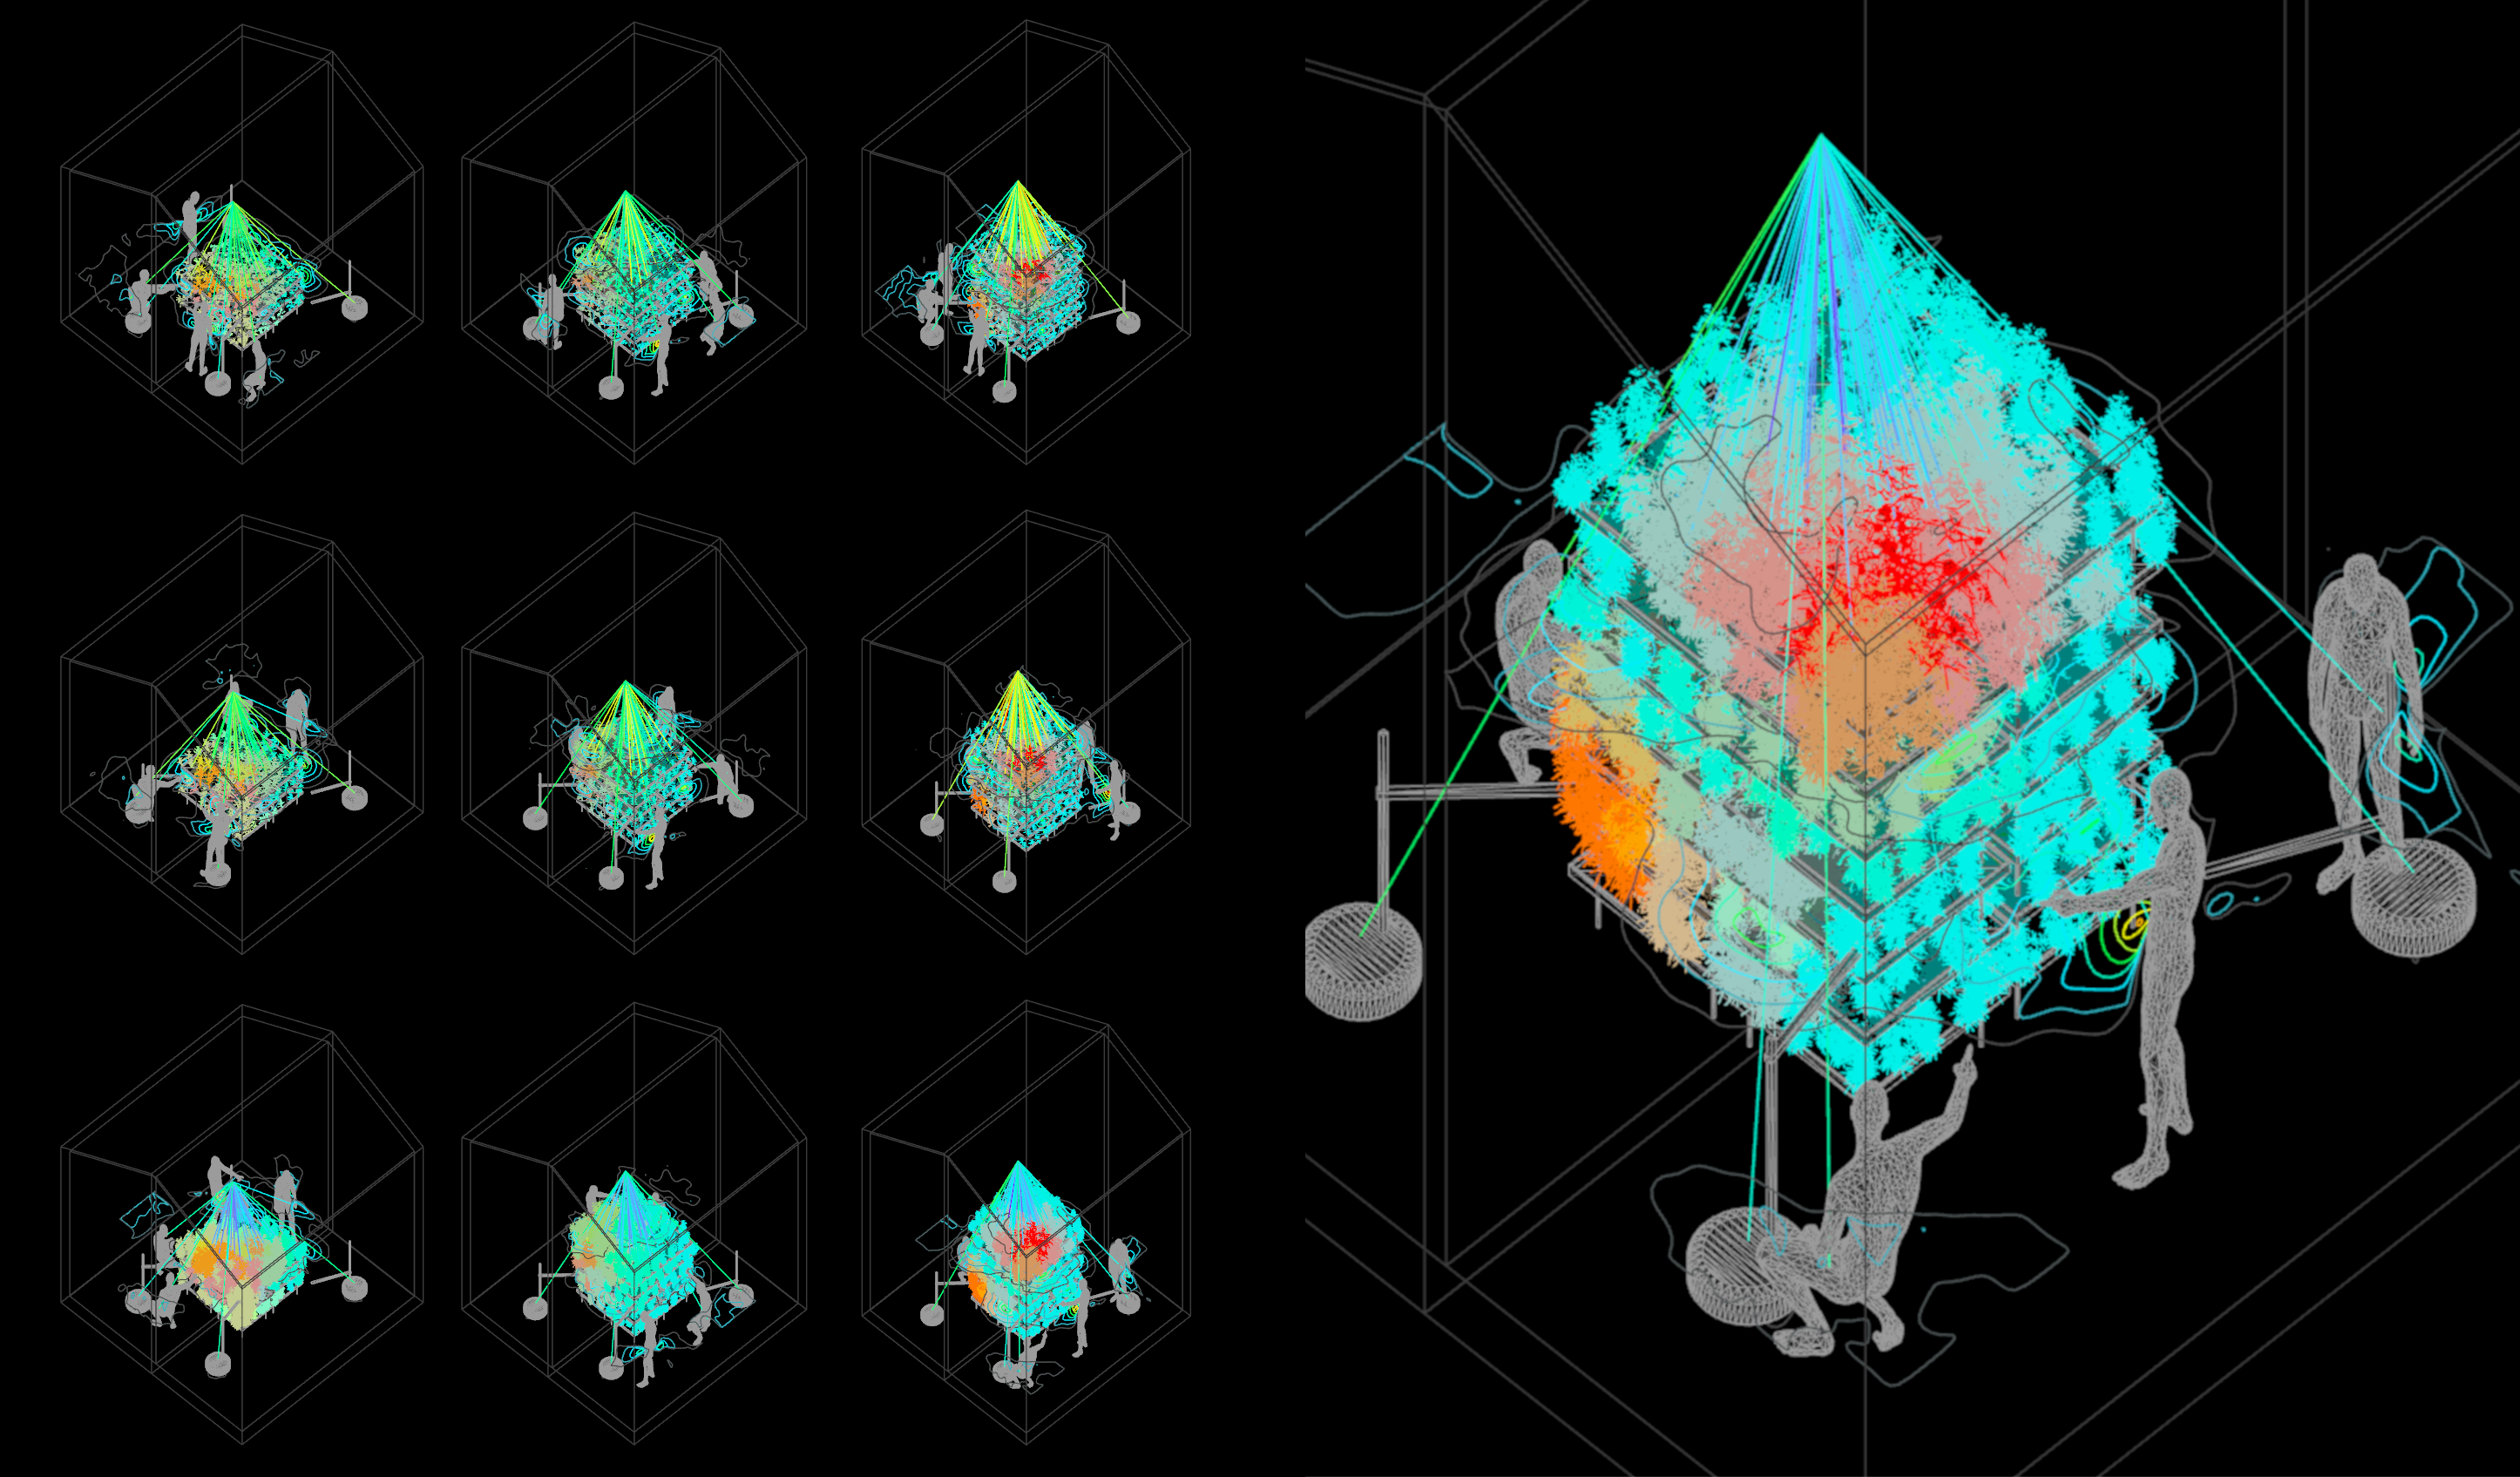
\includegraphics[width=0.98\linewidth]{figures/screenshots/combined3.png}%
    \caption{Procedurally generated cultivation scenes in Houdini, with plants on trays, infrastructure, people, robots, and devices, and the traced paths.}
    \label{fig:scene-example}
\end{figure}

% \begin{figure*}[ht]
\centering
\newcommand{\icon}[1]{\includegraphics[height=7mm]{figures/icons/#1.pdf}}
% Tools (ColorBrewer Dark2, print friendly)
\definecolor{houdini}{HTML}{D95F02}\definecolor{sionna}{HTML}{1B9E77}\definecolor{browser}{HTML}{7570B3}\definecolor{analysis}{HTML}{A6761D}
\begin{tikzpicture}[
  font=\scriptsize,
  node/.style={draw=black!75,fill=white,rounded corners=1pt,align=center,text width=2.3cm,
              minimum height=1.85cm,inner sep=2pt,line width=0.5pt,
              execute at begin node={\hyphenpenalty=10000\exhyphenpenalty=10000}},
  % A step: a white box with a bar in the colour of the tool that performs it
  step/.style={node,path picture={\fill[#1] (path picture bounding box.north west)
              rectangle ([yshift=-2.2pt]path picture bounding box.north east);}},
  output/.style={node,rounded corners=0pt},
  todo/.style={node,draw=black!50,dash pattern=on 2pt off 1.5pt},
  arr/.style={-{Latex[length=1.6mm,width=1.2mm]},line width=0.5pt,black!85},
  todoarr/.style={arr,dash pattern=on 2pt off 1.5pt},
  dot/.style={circle,fill=black!85,inner sep=0pt,minimum size=1.1mm},
  stage/.style={fill=black!7,rounded corners=2pt},
  stagelabel/.style={font=\scriptsize\bfseries,anchor=north west,inner sep=4pt,align=left},
  legend/.style={draw=black!75,fill=white,line width=0.5pt,minimum width=3.4mm,minimum height=2.6mm,inner sep=0pt},
  % The whole box links to the section that describes it.
  link/.style={alias=linked,append after command={
    let \p1=(linked.north west),\p2=(linked.south east),\n1={\x2-\x1},\n2={\y1-\y2} in
    node[inner sep=0pt,outer sep=0pt,anchor=north west] at (\p1)
      {\hyperref[#1]{\phantom{\rule{\n1}{\n2}}}}}},
]
% Stages. The boundaries run through the middle of "Check and export" (1|2) and "Results" (2|3),
% the steps that hand over from one stage to the next.
\fill[stage] (-1.35,1.95) rectangle (2.88,-4.0);
\fill[stage] (3.02,1.95)  rectangle (8.78,-1.25);
\fill[stage] (8.92,1.95) -- (13.2,1.95) -- (13.2,-4.0) -- (7.5,-4.0) -- (7.5,-1.39) -- (8.92,-1.39) -- cycle;
\node[stagelabel,link=sec:procedural] at (-1.35,1.95) {1\enspace Procedural scene generation};
\node[stagelabel,link=sec:raytracing] at (3.02,1.95)  {2\enspace Ray tracing};
\node[stagelabel,link=sec:evaluation] at (8.92,1.95)  {3\enspace Evaluation};

% 1 Procedural scene generation
\node[step=houdini,link=sec:geometry] (proc) at (0,0)
  {\icon{scene}\\[2pt]\textbf{Procedural scene}\\crops, greenhouse, devices};
\node[todo,link=sec:twin] (cal) at (0,-2.9)
  {\icon{calibrate}\\[2pt]\textbf{Calibrate}\\materials and antennas};
% 1|2 and 2 Ray tracing
\node[step=houdini,link=sec:scene] (exp) at (2.95,0)
  {\icon{export}\\[2pt]\textbf{Check and export}\\geometry and materials};
\node[step=sionna,link=sec:execution] (rt) at (5.9,0)
  {\icon{raytrace}\\[2pt]\textbf{Ray tracing}\\ on a GPU or CPU (LLVM backend), local or remote and in batches};
% 2|3 and 3 Evaluation
\node[output,link=sec:returned] (out) at (8.85,0)
  {\icon{results}\\[2pt]\textbf{Results}\\paths, links, radio maps};
\node[step=browser,link=sec:inspection] (view) at (11.8,0)
  {\icon{viewer}\\[2pt]\textbf{Web viewer}\\explore scenes, paths and maps};
\node[step=analysis,link=sec:metrics] (eng) at (8.85,-2.9)
  {\icon{engine}\\[2pt]\textbf{Application engine}\\coverage and RF energy metrics};
\node[step=houdini,link=sec:inspection] (hou) at (11.8,-2.9)
  {\icon{houdini}\\[2pt]\textbf{Inspect in Houdini}\\results on the scene};
% Towards a digital twin, below the ray-tracing stage
\node[todo,link=sec:twin] (meas) at (4.42,-2.9)
  {\icon{measure}\\[2pt]\textbf{Field measurements}\\RF and crop state};

\draw[arr] (proc)--(exp);
\draw[arr] (exp)--(rt);
\draw[arr] (rt)--(out);
\draw[arr] (out)--(view);
\draw[arr] (out.south) -- (8.85,-1.65) node[dot]{} -- (eng.north);
\draw[arr] (8.85,-1.65) -| (hou.north);
% Iteration back to the scene, around the left of the stages
\draw[arr] (view.north) -- (11.8,2.45) -- node[above,inner sep=2pt]
  {\raisebox{\dimexpr 0.55ex-1.1mm\relax}{
\includegraphics[height=2.2mm]{figures/icons/iterate.pdf}}\enspace\textit{iterate: change the scene or sweep parameters}}
  (-1.65,2.45) -- (-1.65,0) -- (proc.west);
% Field measurements are compared with the predictions and calibrate the scene
\draw[todoarr] (meas) -- node[above,inner sep=2pt]{\textit{compare}} (eng);
\draw[todoarr] (meas) -- node[above,inner sep=2pt]{\textit{calibrate}} (cal);
\draw[todoarr] (cal) -- node[left,inner sep=2pt]{\textit{update}} (proc);

% Legend: the tool behind each step
\node[anchor=north west,inner sep=0pt,align=left] at (13.5,1.95) {\textbf{Tool}\\[3pt]
  \tikz\node[legend,path picture={\fill[houdini] (path picture bounding box.north west) rectangle ([yshift=-1.4pt]path picture bounding box.north east);}]{};\enspace Houdini\\[3pt]
  \tikz\node[legend,path picture={\fill[sionna] (path picture bounding box.north west) rectangle ([yshift=-1.4pt]path picture bounding box.north east);}]{};\enspace Sionna RT\\[3pt]
  \tikz\node[legend,path picture={\fill[browser] (path picture bounding box.north west) rectangle ([yshift=-1.4pt]path picture bounding box.north east);}]{};\enspace Browser\\[3pt]
  \tikz\node[legend,path picture={\fill[analysis] (path picture bounding box.north west) rectangle ([yshift=-1.4pt]path picture bounding box.north east);}]{};\enspace Python or other\\[6pt]
  \tikz\node[legend]{};\enspace output data\\[3pt]
  \tikz\node[legend,draw=black!50,dash pattern=on 1.2pt off 0.9pt]{};\enspace not yet implemented};
\end{tikzpicture}
\caption{The \housionna{} workflow in three stages. \emph{Check and export} and \emph{Results} hand over between stages; the bar on each step shows the tool that performs it, and the square box is output data. Dashed elements are needed for an agricultural digital twin, in which field measurements calibrate the materials and antennas of the scene. Each box and stage title links to the section that describes it.}
\label{fig:pipeline}
\end{figure*}


\begin{figure*}[t]
\centering
\newcommand{\icon}[1]{\includegraphics[height=6mm]{figures/icons/#1.pdf}}
\newcommand{\card}[4][sub]{\vspace*{1.5pt}\icon{#2}\\[5pt]\textbf{#3}\\[0.5pt]{\fontsize{6.3}{7.5}\selectfont\color{#1}#4\par}}
\newcommand{\cardw}{2.45cm}\newcommand{\cardh}{1.82cm}
% Tools (jet hues as in the ray-tracing renders)
\definecolor{houdini}{HTML}{FF5A1F}\definecolor{sionna}{HTML}{76B900}\definecolor{browser}{HTML}{6A5BFF}\definecolor{analysis}{HTML}{EBCB00}
\definecolor{ink}{HTML}{000000}\definecolor{sub}{HTML}{595959}\definecolor{frame}{HTML}{A6A6A6}\definecolor{dim}{HTML}{8C8C8C}\definecolor{subdim}{HTML}{B3B3B3}\definecolor{panel}{HTML}{F0F0F0}
\begin{tikzpicture}[
  font=\fontfamily{phv}\selectfont\scriptsize,color=ink,
  every node/.append style={outer sep=0pt},
  card/.style={fill=white,draw=ink,line width=0.4pt,text=ink,inner sep=3pt,
               execute at begin node={\begin{minipage}[c][\cardh][t]{\cardw}\centering
                 \hyphenpenalty=10000\exhyphenpenalty=10000},
               execute at end node={\end{minipage}}},
  % A step: a card with a bar in the colour of the tool that performs it
  bar/.style={path picture={\fill[#1] (path picture bounding box.north west)
               rectangle ([yshift=-2.8pt]path picture bounding box.north east);}},
  step/.style={card,bar=#1},
  output/.style={card},
  % Not yet implemented: only the dashed border marks it, text and icon stay readable
  todo/.style={card,draw=dim,dash pattern=on 2pt off 1.5pt},
  arr/.style={-{Latex[length=1.5mm,width=1.1mm]},line width=0.45pt,ink,shorten >=1.5pt,shorten <=1.5pt},
  todoarr/.style={arr,dim,dash pattern=on 2pt off 1.5pt},
  lbl/.style={font=\fontfamily{phv}\selectfont\scriptsize\itshape,inner sep=2.5pt},
  % Stages are borderless panels, so arrows between stages cross no lines
  stage/.style={fill=panel},
  stagelabel/.style={font=\fontfamily{phv}\selectfont\scriptsize\bfseries,anchor=north west,inner xsep=0.2cm,inner ysep=4pt,align=left},
  num/.style={fill=black,text=white,font=\fontfamily{phv}\selectfont\tiny\bfseries,minimum size=3.2mm,inner sep=0pt},
  swatch/.style={fill=white,draw=ink,line width=0.4pt,minimum width=3.6mm,minimum height=2.6mm,inner sep=0pt},
  % The whole box links to the section that describes it.
  link/.style={alias=linked,append after command={
    let \p1=(linked.north west),\p2=(linked.south east),\n1={\x2-\x1},\n2={\y1-\y2} in
    node[inner sep=0pt,outer sep=0pt,anchor=north west] at (\p1)
      {\hyperref[#1]{\phantom{\rule{\n1}{\n2}}}}}},
]
% Grid: cards 2.66 cm wide, 0.2 cm inside each stage panel, 0.55 cm apart within a stage.
% Columns at x = 1.53, 4.74 | 8.25 | 12.41, 15.62; rows at y = 0 and -3. Every card lies inside one stage;
% the wider gap before stage 3 leaves room for the "compare" label.
\fill[stage] (0,1.6)     rectangle (6.27,-4.22);   % 1: scene and export (Houdini)
\fill[stage] (6.72,1.6)  rectangle (9.78,-1.22);   % 2: ray tracing only, top row
\fill[stage] (10.88,1.6) rectangle (17.15,-4.22);  % 3: results and their use

\node[stagelabel,link=sec:procedural] at (0,1.6)     {\tikz[baseline=(n.base)]\node[num](n){1};\enspace Procedural scene generation};
\node[stagelabel,link=sec:raytracing] at (6.72,1.6)  {\tikz[baseline=(n.base)]\node[num](n){2};\enspace Ray tracing};
\node[stagelabel,link=sec:evaluation] at (10.88,1.6) {\tikz[baseline=(n.base)]\node[num](n){3};\enspace Evaluation};

% 1 Procedural scene generation
\node[step=houdini,link=sec:geometry] (proc) at (1.53,0)  {\card{scene}{Procedural scene}{crops, greenhouse\\and devices}};
\node[step=houdini,link=sec:scene]    (exp)  at (4.74,0)  {\card{export}{Check and export}{geometry and materials}};
\node[todo,link=sec:twin]             (cal)  at (1.53,-3) {\card{calibrate}{Calibrate}{materials and antennas}};
% 2 Ray tracing
\node[step=sionna,link=sec:execution] (rt)   at (8.25,0)  {\card{raytrace}{Ray tracing}{GPU/CPU execution,\\local, remote, batched}};
% 3 Evaluation
\node[output,link=sec:returned]         (out)  at (12.41,0)  {\card{results}{Results}{paths, links, radio maps}};
\node[step=browser,link=sec:inspection] (view) at (15.62,0)  {\card{viewer}{Web viewer}{explore scenes,\\paths and maps}};
\node[step=analysis,link=sec:metrics]   (eng)  at (12.41,-3) {\card{engine}{Application engine}{coverage and\\RF energy metrics}};
\node[step=houdini,link=sec:inspection] (hou)  at (15.62,-3) {\card{houdini}{Inspect in Houdini}{results on the scene}};
% Towards a digital twin: outside the stages, below ray tracing
\node[todo,link=sec:twin]               (meas) at (8.25,-3)  {\card{measure}{Field measurements}{RF and crop state}};

\draw[arr] (proc)--(exp);
\draw[arr] (exp)--(rt);
\draw[arr] (rt)--(out);
\draw[arr] (out)--(view);
% Results feed both the application engine and Houdini: two arrows, no junction
\draw[arr] (out.south) -- (eng.north);
\draw[arr] ([xshift=5mm]out.south) |- (15.62,-1.5) -- (hou.north);

% Iteration back to the scene, from the top of the evaluation stage
\draw[arr] (14.015,1.6) -- (14.015,2.1)
  -- node[lbl,above]{\raisebox{\dimexpr 0.55ex-1.2mm\relax}{
\includegraphics[height=2.4mm]{figures/icons/iterate.pdf}}\enspace iterate: change the scene or sweep parameters}
  (-0.4,2.1) -- (-0.4,0) -- (proc.west);

% Field measurements: compared with the predictions, then calibrate the scene
\draw[todoarr] (meas) -- node[lbl,above,ink,pos=0.42]{compare} (eng);
\draw[todoarr] (meas) -- node[lbl,above,ink,pos=0.62]{calibrate} (cal);
\draw[todoarr] (cal) -- node[lbl,left,ink]{update} (proc);

% Legend: tools | output and status
\node[anchor=north,inner sep=0pt] at (8.375,-4.5) {\textbf{Tool}\quad
  \raisebox{-0.35mm}{\tikz\node[swatch,bar=houdini]{};}\enspace Houdini\quad
  \raisebox{-0.35mm}{\tikz\node[swatch,bar=sionna]{};}\enspace Sionna RT\quad
  \raisebox{-0.35mm}{\tikz\node[swatch,bar=browser]{};}\enspace Browser\quad
  \raisebox{-0.35mm}{\tikz\node[swatch,bar=analysis]{};}\enspace Python or other
  \qquad\textcolor{frame}{\rule[-0.5mm]{0.4pt}{3.5mm}}\qquad
  \raisebox{-0.35mm}{\tikz\node[swatch]{};}\enspace Output data\quad
  \raisebox{-0.35mm}{\tikz\node[swatch,draw=dim,dash pattern=on 1.2pt off 0.9pt]{};}\enspace Not yet implemented};
\end{tikzpicture}
\caption{The \housionna{} workflow in three stages. The bar on each step shows the tool that performs it; the box without a bar is output data. Dashed elements are needed for an agricultural digital twin, in which field measurements calibrate the materials and antennas of the scene. Each box and stage title links to the section that describes it.}
\label{fig:pipeline}
\end{figure*}


These applications impose different RF requirements. Active telemetry needs sufficient link margin, and batteryless operation also requires enough harvested energy per observation. Backscatter reduces the need for a sensor node to generate its own carrier~\cite{liu2013}, but requires both illumination and a return link to the gateway. Distributed \gls{wpt} depends on spatial channels and coherent combining~\cite{callebaut2024}. The propagation channel can also provide observations of the environment, as illustrated by radio tomography~\cite{wilson2010}; relating channel changes to crop conditions requires crop-specific models and independent reference measurements.

The cultivation environment affects all these links. Leaves, stems, growing trays, support structures, and greenhouse surfaces alter line-of-sight visibility and multipath. Growth changes the geometry, while water content changes the electromagnetic properties of plant tissue. Measurements in a tomato greenhouse show substantial differences from conventional propagation models~\cite{cama2019}. Deployment analysis therefore needs site-specific channels and should account for changes in the crop, device positions, and infrastructure.

Parameterised models can vary species, growth stage, spacing, leaf water content, room layout, occupancy, gateway density, and device placement without rebuilding each scene. Controlled sweeps then change selected properties while the others stay fixed, exposing placements that work for one crop configuration but fail as the canopy develops.
   

Existing workflows also address scene preparation and integration with Sionna RT. SionnaRT-Bridge connects Blender scene preparation, radio-material assignment, transmitter and receiver configuration, Sionna RT simulation, and result visualisation~\cite{ribas2026sionnartbridge}. SceneBaker generates Sionna RT-ready scenes programmatically from map and terrain data~\cite{lyu2026scenebaker}. Neither generates crop geometry or sweeps crop growth.

This paper presents \housionna{}, a workflow connecting procedural scene generation in Houdini with GPU-accelerated radio ray tracing in Sionna RT~\cite{housionna}. Its contribution is the combination of parameterised agricultural geometry, controlled crop and infrastructure sweeps, and analysis of sensor coverage and RF energy harvesting. The workflow integrates scene preparation and export, batch execution, run provenance, and inspection of paths, link metrics, and radio maps in Houdini or a web viewer; Sionna RT provides the electromagnetic solver~\cite{hoydis2023,aoudia2025}. A batteryless plant-sensor use case brings these stages together to examine connectivity, charge time, and the choice of harvester.

\Cref{fig:pipeline} outlines the workflow, and \cref{fig:scene-example} shows example scenes. \Cref{sec:procedural,sec:raytracing,sec:evaluation} describe procedural scene generation, ray tracing, and evaluation, respectively. \Cref{sec:casestudy} applies the workflow to the plant-sensor use case, and \cref{sec:conclusion} discusses limitations and the steps towards an agricultural digital twin.




\FloatBarrier\section{Procedural Scene Generation}
\label{sec:procedural}
\label{sec:simulator}
% The first stage of \housionna{} constructs the agricultural environment in Houdini. A parameterised node network generates geometry, assigns material attributes, and places gateways, sensor nodes, and measurement surfaces for the ray-tracing stage. It can represent alternative crop layouts or infrastructure configurations without manually rebuilding every scene.


The first stage of  \housionna{}  constructs the agricultural environment in Houdini 22, a proprietary procedural modelling tool (the free non-commercial edition suffices) in which each scene is the output of a node network rather than a manually edited model. Exposed parameters control crop species, growth stage, plant spacing, room size, infrastructure, occupancy, and device density. The network generates the geometry and assigns material attributes per primitive (material, thickness, and water content), so these properties can vary within one scene. Measurement surfaces for radio maps are added the same way. Scene generation is deterministic: random choices use explicit seeds, so a scene is fully defined by its parameter values and can be regenerated exactly from them. Batches are organised with Houdini’s Procedural Dependency Graph (PDG), which turns combinations of parameter values into work items, each producing one scene variant (\cref{sec:execution}). Alternative crop layouts and infrastructure configurations therefore do not have to be rebuilt by hand, and every result can be traced back to the parameters that generated its scene.





% \subsection{Agricultural Geometry}\label{sec:geometry}
% The scene parameters include plant spacing, canopy height and depth, leaf orientations, infrastructure layout, and device positions; gateways and sensor nodes can be placed anywhere, including on plants and on mobile robots. Plants are generated with L-systems in three growth stages, optionally with fruit, so growth is represented by a sequence of static scenes. People, autonomous robots, windows, and metal frames can be added as disturbances of the channel. A geometric growth parameter is not automatically a validated physiological model. \Cref{fig:growth_stages} illustrates the three growth stages. \gilles{be sure to mention where these models are coming from.}






\subsection{Agricultural Geometry}\label{sec:geometry}
Plants are generated with L-systems, using Houdini's L-system operator. Species-specific rules, written for this work and included in the repository~\cite{housionna}, produce five growth stages (0--4) per species, optionally with fruit. Growth is therefore represented by a sequence of static scenes; the stages are geometric snapshots, not a validated physiological growth model. \Cref{fig:growth_stages} shows the five growth stages of cherry tomato. Leaves are single surfaces rather than closed volumes, and their slab thickness is a material attribute (\cref{sec:materials}), so paths through them are not lost to the \SI{1}{cm} segment limit (\cref{sec:solver}). Plants are placed on trays at a set spacing, in a room of parametric size with its structural frame, windows, sprayers, and secondary structure. People and robots are added as disturbances of the channel; an occupancy parameter and a seed set their number and positions.

Gateways and sensor nodes are points carrying their role, transmit power, antenna pattern, polarisation, and orientation. Each sensor node is attached to its plant at a seeded position, at a clearance of \SI{2}{cm} from leaves, stems, and trays, and stays attached through the growth stages. Like a physical sensor, it moves with the plant, and its orientation follows the main stem, so the antenna axis and polarisation change as the plant grows. Gateways are distributed evenly over a horizontal plane above the crop at a set density per floor area, with at least one, and face downwards. Devices can also be mounted on robots or people as mobile nodes.
   
% \begin{figure*}[htp]
% \centering
% \newcommand{\gridimg}[2]{%
%   \begin{minipage}[t]{0.19\linewidth}\raggedright
%     \includegraphics[width=\linewidth]{figures/procedural/#1_#2}\\
%     {\scriptsize x=#1\\y=#2\par}
%   \end{minipage}}%
% \newcommand{\gridrow}[1]{%
%   \gridimg{0}{#1}\hfill\gridimg{1}{#1}\hfill\gridimg{2}{#1}\hfill\gridimg{3}{#1}\hfill\gridimg{4}{#1}\par\smallskip}%
% \gridrow{0}
% \gridrow{1}
% \gridrow{2}
% \caption{Procedural scene variations.}
% \label{fig:procedural_matrix}
% \end{figure*}



% \begin{figure*}[htp]
% \centering
% \newcommand{\gridimg}[2]{%
%   \begin{minipage}[t]{0.19\linewidth}\raggedright
%     \includegraphics[width=\linewidth]{figures/procedural/#1_#2}\\
%     {\scriptsize sensors=#1\\y=#2\par}
%   \end{minipage}}%
% \newcommand{\gridrow}[1]{%
%   \gridimg{0}{#1}\hfill\gridimg{1}{#1}\hfill\gridimg{2}{#1}\hfill\gridimg{3}{#1}\hfill\gridimg{4}{#1}\par\smallskip}%
% \gridrow{0}
% \gridrow{1}
% \gridrow{2}
% \caption{Procedural scene variations.}
% \label{fig:procedural_matrix}
% \end{figure*}


% \begin{figure}[ht]
% \centering
% \newcommand{\stageimg}[1]{%
%   \begin{minipage}[t]{0.32\linewidth}\raggedright
%     \includegraphics[width=\linewidth]{figures/growth_stage/#1}\\[-1pt]
%     {\scriptsize #1\par}
%   \end{minipage}}%
% \stageimg{seedling}\hfill\stageimg{vegetative}\hfill\stageimg{mature}
% \caption{Plant growth stages.}
% \label{fig:growth_stages}
% \end{figure}



% testing

% \begin{figure}[ht]
% \centering
% \stageimg{ocimum_basilicum_v1_gen1}{Gen.~1}\hfill\stageimg{ocimum_basilicum_v1_gen2}{Gen.~2}\hfill\stageimg{ocimum_basilicum_v1_gen3}{Gen.~3}
% \caption{\textit{Ocimum basilicum}, variant 1.}
% \label{fig:ocimum_v1}
% \end{figure}

% \begin{figure}[ht]
% \centering
% \stageimg{ocimum_basilicum_v2_gen1}{Gen.~1}\hfill\stageimg{ocimum_basilicum_v2_gen2}{Gen.~2}\hfill\stageimg{ocimum_basilicum_v2_gen3}{Gen.~3}
% \caption{\textit{Ocimum basilicum}, variant 2.}
% \label{fig:ocimum_v2}
% \end{figure}

% \begin{figure}[ht]
% \centering
% \stageimg{ocimum_basilicum_v3_gen1}{Gen.~1}\hfill\stageimg{ocimum_basilicum_v3_gen2}{Gen.~2}\hfill\stageimg{ocimum_basilicum_v3_gen3}{Gen.~3}
% \caption{\textit{Ocimum basilicum}, variant 3.}
% \label{fig:ocimum_v3}
% \end{figure}

% \newcommand{\stageimg}[2]{%
%   \begin{minipage}[t]{0.32\linewidth}\raggedright
%     \includegraphics[width=\linewidth]{figures/growth_stage/#1}\\[-1pt]
%     {\scriptsize #2\par}
%   \end{minipage}}

% \begin{figure}[t]
% \centering
% \stageimg{fragaria_x_ananassa_v1_gen1}{Gen.~1}\hfill\stageimg{fragaria_x_ananassa_v1_gen2}{Gen.~2}\hfill\stageimg{fragaria_x_ananassa_v1_gen3}{Gen.~3}\\[2pt]
% \stageimg{solanum_lycopersicum_v1_gen1}{Gen.~1}\hfill\stageimg{solanum_lycopersicum_v1_gen2}{Gen.~2}\hfill\stageimg{solanum_lycopersicum_v1_gen3}{Gen.~3}
% \caption{Three generated growth stages of strawberry (\textit{Fragaria $\times$ ananassa}, top) and tomato (\textit{Solanum lycopersicum}, bottom).}
% \label{fig:growth_stages}
% \end{figure}





\newcommand{\stageimg}[2]{%
  \begin{minipage}[t]{0.31\linewidth}\raggedright
    \includegraphics[width=\linewidth]{figures/growth_stage/#1}\\[-1pt]
    {\scriptsize #2\par}
  \end{minipage}}

% \begin{figure}[ht]
% \centering
% \stageimg{fragaria_x_ananassa_v1_gen1}{Gen.~1}\hfill\stageimg{fragaria_x_ananassa_v1_gen2}{Gen.~2}\hfill\stageimg{fragaria_x_ananassa_v1_gen3}{Gen.~3}\\[2pt]
% \stageimg{solanum_lycopersicum_v1_gen1}{Gen.~1}\hfill\stageimg{solanum_lycopersicum_v1_gen2}{Gen.~2}\hfill\stageimg{solanum_lycopersicum_v1_gen3}{Gen.~3}
% \caption{Three generated growth stages of strawberry (\textit{Fragaria $\times$ ananassa}, top) and tomato (\textit{Solanum lycopersicum}, bottom).}\label{fig:growth_stages}
% \end{figure}




\begin{figure}[hbtp]
    \centering
    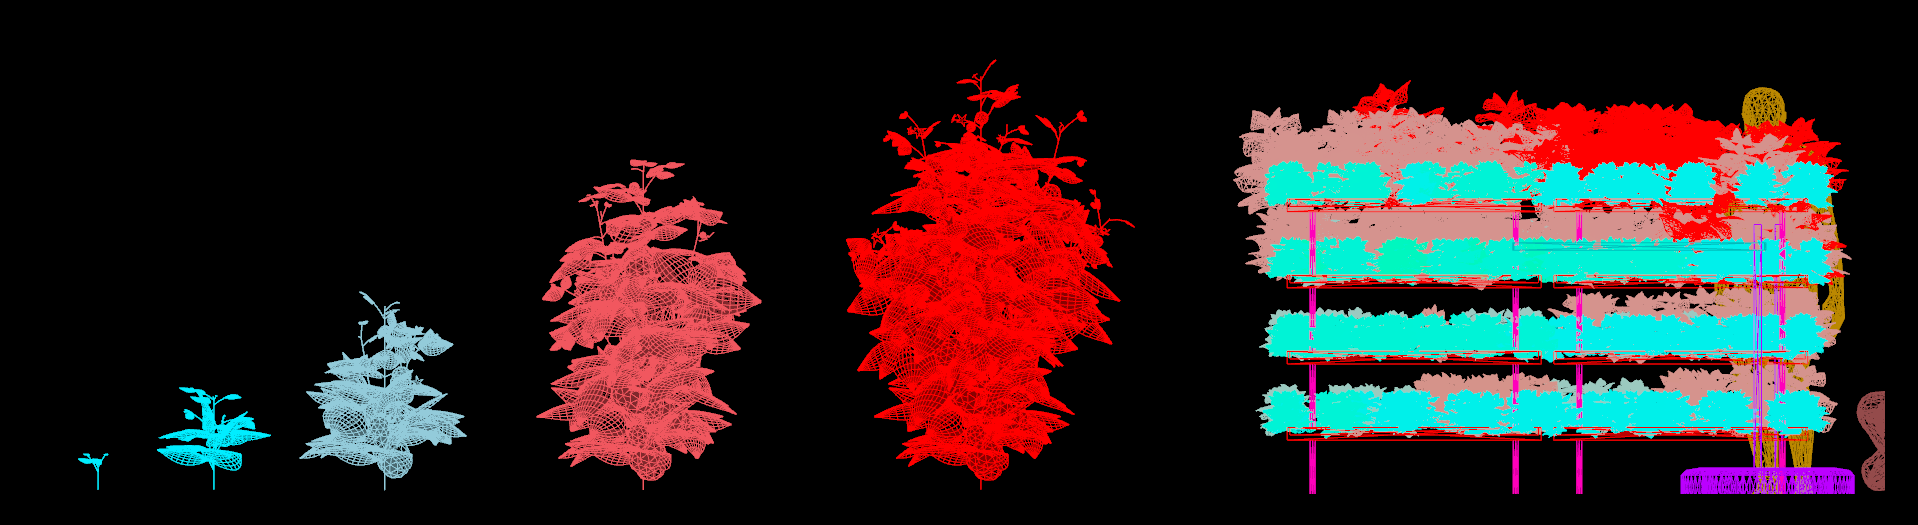
\includegraphics[width=0.98\linewidth]{figures/screenshots/combined5.png}%
    % 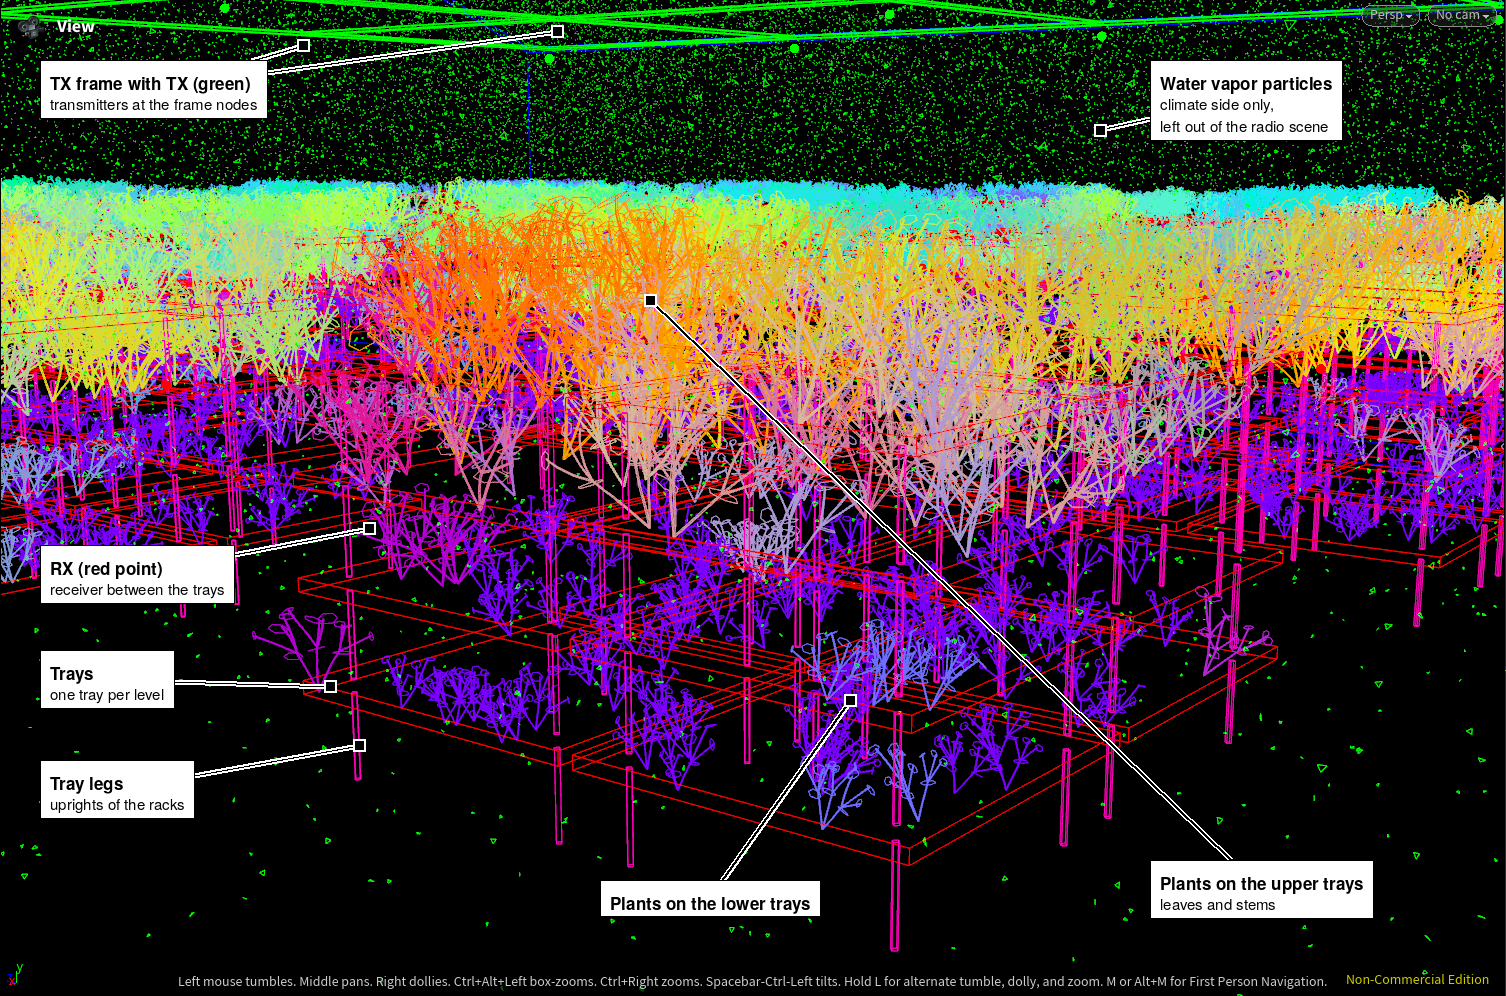
\includegraphics[width=0.5\linewidth]{figures/procedural/annotated_00bbc1c9.png}
    \caption{Five generated growth stages and one rack of cherry tomato (\textit{Solanum lycopersicum}).}\label{fig:growth_stages}
\end{figure}




% \subsection{Radio Materials}\label{sec:materials}
% The built-in ITU-R P.2040 materials of Sionna are bounded in frequency~\cite{itu2040}: apart from wood and glass, they are defined only from \SI{1}{GHz}, which excludes the \SI{868}{MHz} and \SI{915}{MHz} bands. \housionna{} therefore adds frequency-dependent models and records a source and status for each material: Cole--Cole fits of common building materials measured from \SIrange{0.2}{67}{GHz}~\cite{zhekov2020}, conductors for metal structures, water and nutrient solution~\cite{liebe1991}, soils~\cite{itu527}, and the dual-dispersion vegetation model for leaves and stems~\cite{ulaby1987}. The vegetation coefficients are not yet verified, and fruit and growing media use placeholder values, so plant materials must be treated as provisional. ITU-R P.833 provides an independent vegetation-attenuation reference for appropriate scenarios~\cite{itu833}; it does not replace calibration for the specific crop and geometry.


\subsection{Radio Materials}\label{sec:materials}
The built-in ITU-R P.2040 materials of Sionna are bounded in frequency~\cite{itu2040}: apart from wood and glass, they are defined only from \SI{1}{GHz}, which excludes the \SI{868}{MHz} and \SI{915}{MHz} bands. \housionna{} therefore adds frequency-dependent models and records a source, status, and valid frequency range for each material, with a warning when a run extrapolates beyond that range. The models are Cole--Cole fits of common building materials measured from \SIrange{0.2}{67}{GHz}~\cite{zhekov2020}, conductors for metal structures, water and nutrient solution~\cite{liebe1991}, soils~\cite{itu527}, the dual-dispersion vegetation model for leaves~\cite{ulaby1987}, and a four-term Cole--Cole model of dry skin for people~\cite{gabriel1996}. Material properties are evaluated at the frequency of each run or work item. Material, slab thickness, and water content are primitive attributes, so water content (\% of fresh mass for leaves, default \SI{80}{\percent}; \% of volume for soils) can vary within a scene and across work items. Leaves use an assumed slab thickness of \SI{0.3}{mm}. The vegetation model is not validated for the crops considered here, and fruit and growing media use placeholder values, so plant materials must be treated as provisional. ITU-R P.833 provides an independent vegetation-attenuation reference for appropriate scenarios~\cite{itu833}; it does not replace calibration for the specific crop and geometry.


\section{Ray Tracing}
\label{sec:raytracing}
The second stage transfers the procedural scene to Sionna RT, computes propagation paths and radio maps, and records each run for subsequent inspection and analysis.




\subsection{Scene Checks and Export}
\label{sec:scene}
The exporter groups triangular geometry by object name and writes meshes, a scene description, material parameters, device definitions, and solver settings.

Export checks include triangulation, object names, material consistency, and device definitions. These are checks of simulation input integrity; they do not establish biological realism or material accuracy. A preview stage loads the exported scene in Sionna and returns its geometry for inspection in Houdini.

% \subsection{Solver Configuration and Geometry Interactions}
% The current implementation uses Sionna RT 2.2.0 and a single isotropic, vertically polarised antenna at each gateway and sensor node~\cite{housionna}. The solver accepts controls for line of sight, specular and diffuse reflection, transmission/refraction, diffraction, interaction depth, and sampling budgets. Enabling an interaction does not guarantee that a chosen scene representation models the corresponding canopy physics accurately.

% Sionna models interactions with surfaces: each surface a ray crosses acts as a slab with the full thickness of its radio material. A closed canopy shell, internal sheets, and explicit leaf geometry can produce different depth-dependent attenuation. Refining the mesh alone does not resolve this modelling choice. When a leaf or stem is small relative to wavelength, a surface ray approximation may miss relevant scattering behaviour. Sionna RT also discards paths containing a segment shorter than \SI{1}{cm}, so every path through a closed leaf or stem thinner than this is lost. The slab behaviour and the \SI{1}{cm} limit were confirmed with analytical reference cases (free space, a single slab, a closed block, and thin glass) included in the repository~\cite{housionna}. Representation and material uncertainty must be assessed together.



\subsection{Solver Configuration and Geometry Interactions}\label{sec:solver}
The implementation uses Sionna RT 2.2.0. Antenna pattern (isotropic, short dipole, half-wave dipole, or the 3GPP TR 38.901 element pattern~\cite{tr38901}) and polarisation are set per device role, as Sionna RT uses one antenna array for all transmitters and one for all receivers; orientation is set per device. The solver accepts controls for line of sight, specular and diffuse reflection, refraction, diffraction, interaction depth, sampling budget, and random seed. Enabling an interaction does not guarantee that the scene representation models the corresponding canopy physics accurately.

Sionna models interactions with surfaces: each surface a ray crosses acts as a slab with the full thickness of its radio material and counts as one interaction, so the depth limit bounds the number of leaves a path can cross. A closed canopy shell, internal sheets, and explicit leaf geometry produce different depth-dependent attenuation, and refining the mesh alone does not resolve this choice. When a leaf or stem is small relative to the wavelength, the surface approximation may miss relevant scattering. Sionna RT also discards paths with a segment shorter than \SI{1}{cm}, so paths through closed objects thinner than this are lost; leaves are therefore single surfaces (\cref{sec:geometry}). Radio maps apply this limit only to diffraction, so thin closed objects can affect paths and radio maps differently. The slab behaviour and the \SI{1}{cm} limit were confirmed with analytical reference cases included in the repository~\cite{housionna}. Representation and material uncertainty must be assessed together.

\subsection{Execution and Reproducibility}\label{sec:execution}
The solver runs in a separate Python environment, locally on a GPU or CPU or on a remote GPU host. A batch process solves each PDG work item in its own process and skips items already solved with the same settings. Run records store the exported scene, resolved materials, devices, solver settings including the seed, the work-item parameters, and software versions, so each result can be traced to its inputs.


% \subsection{Execution and Reproducibility}
% \label{sec:execution}
% The solver runs in a separate Python environment, locally on an NVIDIA GPU or a CPU under Linux, or on a remote GPU host. Results are written as compressed NumPy arrays for the evaluation stage. This separation allows the modelling workstation and compute machine to differ.

% For parameter sweeps, Houdini task-operator (TOP) work items, one per parameter combination, are exported to individual run folders. A background batch process solves work items sequentially within one Sionna session. Successful items can be skipped when their recorded solver settings match, and failed items are recorded for later retry.

% Run records include the exported scene, resolved material properties, devices, settings, a solver copy, and software provenance. Batch records also preserve work-item parameters. Recording these assets makes the simulated geometry inspectable even after the procedural node network has changed. The records do not yet include the random seed of the path solver or hardware details, which a complete release should add.


% \subsection{\texorpdfstring{\protect\hl{Execution and Reproducibility}}{Execution and Reproducibility}}\label{sec:execution}
% \hl{The solver runs in a separate Python environment, locally on an NVIDIA GPU or a CPU, or on a remote GPU host over SSH, so the modelling workstation and the compute machine can differ. Results are written as compressed NumPy arrays for the evaluation stage.}

% \hl{For parameter sweeps, PDG work items, one per parameter combination, are exported to individual run folders. Each work item carries the parameter values of its variant, which drive both the scene network and the solver settings, such as growth stage and frequency in the use case (\cref{sec:usecase}). Together with the seeds, these values fully define the run. A background batch process solves each work item in its own process, so a failure ends only that item. When GPU memory runs out, the transmitters are split into smaller groups and the item is restarted; paths are unaffected, and radio maps differ only by sampling noise. Items whose recorded settings match are skipped, and failed items are recorded for later retry.}

% \hl{Run records include the exported scene, resolved material properties, devices, settings including the random seed, a solver copy, and software provenance (code commit, Houdini, Sionna RT, and Mitsuba versions). Batch records also store the work-item parameters and the machine that solved them. These records keep the simulated geometry inspectable after the procedural network has changed. The GPU model is not yet recorded, and results can differ slightly between GPU and CPU.}

\section{Evaluation}
\label{sec:evaluation}
The third stage makes the simulated channels available for inspection and application analysis. Results can be examined in Houdini or in a web viewer, while an application engine converts the propagation outputs into relevant application metrics, e.g., coverage and energy metrics. 

\subsection{Returned Quantities}
\label{sec:returned}
Propagation paths are imported as polylines carrying gateway and sensor node identifiers, complex amplitudes, delays, interaction types, and object associations. Per-link outputs include path counts, coherent and incoherent gains, RMS delay spread, and frequency-response magnitudes. Radio maps provide path gain per gateway over triangular measurement surfaces. Radio maps average power over cells and do not retain phase, but under maximum-ratio transmission the local mean RF power at the sensor node is $P_{\mathrm{GW}}\sum_i g_{ij}$, where $P_{\mathrm{GW}}$ is the total RF power budget of the gateways. Mean RF power can therefore be evaluated over an area from the per-gateway maps. Maximum-ratio transmission assumes ideal channel knowledge at all gateways and is an upper bound for distributed operation~\cite{callebaut2024}.

% The distinction between link and map outputs matters. Coherent link quantities depend on relative path phase and can vary over small spatial displacements. Radio maps average power over cells and do not retain the phase information required for coherent \gls{wpt} from multiple gateways. Nor does a map of the strongest gateway represent the combined field of several synchronised gateways. Per-gateway maps can nevertheless be combined: with maximum-ratio transmission, the RF power at the sensor node equals the total gateway RF power times the sum of the per-gateway gains, so its local average follows from the maps without phase information. The application engine in \cref{sec:metrics} uses this to evaluate strategies for multiple gateways over an area, and the link outputs to evaluate them at individual sensor nodes.

\subsection{Visual Inspection and Run Browsing}
\label{sec:inspection}
The compressed result arrays are imported into Houdini as attributed geometry, allowing paths and radio maps to be inspected in the original scene. A web viewer built on three.js displays the same paths, radio maps, and link metrics without a Houdini installation, steps through the runs of a batch, and can be published as a read-only website, as for the use-case results of \cref{sec:casestudy}~\cite{housionna}.

\subsection{Application Engine and Metrics}\label{sec:metrics}
The application engine converts the raw RF propagation channels between gateways and sensor nodes into metrics relevant for different applications and technologies.

\subsubsection{Radio Coverage}
Coverage can be evaluated at specified sensor locations or over a measurement surface using Sionna RT's radio map solver.

\emph{Per-link evaluation:} explicit sensor nodes are placed at candidate sensing locations, including on leaves or within the canopy. The path solver returns the paths between each gateway and each sensor node, with the configured antenna patterns and orientations. For crop configuration $s$, the incoherent power gain from gateway $i$ to sensor node $j$ is
\begin{equation}
 g_{ij}^{(s)}=\sum_k\left|a_{ijk}^{(s)}\right|^2,
 \label{eq:coveragegain}
\end{equation}
where $a_{ijk}^{(s)}$ is the coefficient of path $k$. The effective path loss to the gateway with the largest gain is $L_{\mathrm{best},j}^{(s)}=-10\log_{10}\!\left(\max_i g_{ij}^{(s)}\right)$ in decibels. Summing path powers omits their phase cross terms, so this metric excludes fast fading. The complex path coefficients and delays can instead be used to reconstruct the coherent channel and examine constructive and destructive interference at a particular sensor position. Per-link evaluation therefore supports detailed checks of actual mounting positions and antenna orientations, but assesses only the sensor node locations supplied to the solver.

\emph{Radio maps:} the solver estimates the average incoherent path gain from each gateway over cells of a measurement surface~\cite{aoudia2025}. Sionna supports rectangular cells on a plane or triangular cells on a mesh; \housionna{} uses the latter. This provides an overview of candidate deployment regions without placing an explicit sensor node at every location. Coarse cells can conceal local shadowing, whereas finer cells resolve smaller features but require more ray samples for stable estimates.\footnote{A cell average does not establish that every location within that cell is covered, and reducing the cell size does not restore multipath phase interference. Moreover, Sionna RT's radio maps do not apply the configured sensor node antenna pattern or combining vector~\cite{sionnaRadioMaps}. Their gains must therefore be interpreted with care when assessing a plant-mounted antenna with a particular orientation or polarisation.}

For either approach, coverage requires a device-specific link budget. Using the selected point gain or cell-average gain, the link margin is
 \begin{equation}
  M_{ij}^{(s)}=P_{\mathrm{GW},i}+10\log_{10}g_{ij}^{(s)}
        -S_j-L_{\mathrm{impl}}-M_{\mathrm{reserve}},
  \label{eq:margin}
 \end{equation}
where $P_{\mathrm{GW},i}$ and sensor node sensitivity $S_j$ are in dBm (by reciprocity, the uplink uses the sensor node power and gateway sensitivity), and $L_{\mathrm{impl}}$ and $M_{\mathrm{reserve}}$ are implementation losses and a design reserve in decibels. A non-negative margin indicates coverage under these assumptions. When gateway powers differ, the best gateway maximises the margin rather than the path gain alone.

Across a set of crop configurations, the worst margin $\min_s\min_j\max_i M_{ij}^{(s)}$ tests whether every sensor location has an adequate gateway in every simulated configuration.

% \subsubsection{RF Power and Gateway Strategies}
% For independent or time-separated sources, RF powers at a sensor node may be combined under the corresponding averaging assumptions. Coherent operation with multiple gateways instead requires
% \begin{equation}
%  P_{\mathrm{RF},j}=\left|\sum_i h_{ij}w_i\right|^2,
%  \qquad \sum_i |w_i|^2=P_{\mathrm{GW}},
%  \label{eq:wpt}
% \end{equation}
% where $h_{ij}=\sum_k a_k e^{-\mathrm{j}2\pi f\tau_k}$ is the narrowband channel, summed coherently over the paths with amplitudes $a_k$ and delays $\tau_k$,\footnote{The path coefficients of Sionna RT exclude the propagation phase, so the factor $e^{-\mathrm{j}2\pi f\tau_k}$ must be applied explicitly.} and $w_i$ is a gateway weight with units $\sqrt{\mathrm{W}}$.
% With $N$ gateways and the same total power $P_{\mathrm{GW}}$, the engine compares four strategies: all power on the best gateway, $P_{\mathrm{GW}}\max_i|h_{ij}|^2$; an equal split without phase alignment, $(P_{\mathrm{GW}}/N)\sum_i g_{ij}$; an equal split with identical weights and no channel knowledge, $(P_{\mathrm{GW}}/N)|\sum_i h_{ij}|^2$; and maximum-ratio transmission (MRT) with $w_i\propto h_{ij}^*$, which gives $P_{\mathrm{GW}}\sum_i|h_{ij}|^2$. MRT assumes ideal channel knowledge at all gateways and focuses the power on one sensor node at a time, so it is an upper bound for distributed operation~\cite{callebaut2024}. Each gateway has a single isotropic antenna; arrays per gateway and the validation of simulated phases remain future work.

\subsubsection{Energy Harvesting over RF}
For \gls{wpt}, RF power at a sensor node must be combined with a measured rectifier or harvester response. Practical responses are nonlinear, with an operating threshold, power-dependent conversion efficiency, and saturation at high input powers~\cite{boshkovska2015}. Measurements~\cite{ambient6g} can parameterise $F_{\mathrm{EH}}(P_{\mathrm{RF}},f)$, which maps RF input power and frequency to usable DC power under specified load conditions.

During charging, the changing buffer voltage can also affect the conversion response~\cite{wagih2021}. For a given waveform and harvester, we therefore include the buffer voltage $V_{\mathrm{buf}}(t)$ in the response and write the charging energy balance as
\begin{equation}
 \int_0^T F_{\mathrm{EH}}\!\left(P_{\mathrm{RF}}(t),f,V_{\mathrm{buf}}(t)\right)\,dt
 \geq \Delta E_{\mathrm{buf}}+E_{\mathrm{loss}}(T),
 \label{eq:energy}
\end{equation}
where $\Delta E_{\mathrm{buf}}$ is the required increase in stored energy from the initial state to the target operating level, sufficient for a measurement-and-transmission cycle. $E_{\mathrm{loss}}(T)$ accounts for leakage and quiescent consumption not already included in $F_{\mathrm{EH}}$.

The charge time is the earliest $T$ satisfying this balance and the harvester's startup requirements. Because the response is nonlinear, evaluating it at the average RF input power generally gives a different result from averaging the harvested power. Charging estimates should therefore follow the RF power and buffer state over time. For a static channel and a response measured at a single output voltage, as for datasheet curves, the balance reduces to a constant-power charge time $T=\Delta E_{\mathrm{buf}}/F_{\mathrm{EH}}(P_{\mathrm{RF}},f)$, an approximation used in \cref{sec:casestudy}.

% \subsubsection{Gateway Placement}
% Candidate gateway subsets are compared using the precomputed channels, applying the same communication and energy requirements to each subset. Reporting the preferred subset for each number of gateways shows whether the locations that support connectivity also provide sufficient RF power. The comparison uses the coverage criterion in \eqref{eq:worstmargin} and the reporting intervals derived from \eqref{eq:energy}. Candidate positions, the number of active gateways, and the required margins or reporting intervals are specified for each deployment.

% \subsubsection{Backscattering}
% The gains from the illuminating device to the sensor node and from the sensor node to the gateway follow from a single run. Paths are computed from the illuminating device \gilles{sensor node or gateway?} and the gateway to the sensor nodes; reciprocity provides the reverse link from each sensor node to the gateway. A simple narrowband bistatic model is
% \begin{equation}
%  P_{\mathrm{mod},i}\approx P_{\mathrm{ill}}\,
%  g_{\mathrm{ill},j}\,g_{j,i}\,\eta_{\mathrm{mod}},
%  \label{eq:backscatter}
% \end{equation}
% where $j$ identifies the sensor node, $i$ the gateway, and $\eta_{\mathrm{mod}}$ the effective differential modulation of the sensor node under consistent antenna normalisation. The engine does not yet implement a modulating backscatter sensor node; a backscatter study needs a scattering model for the sensor node, polarisation, gateway noise, the direct illuminating signal, and validation against the deployed geometry.

% \section{Validation Protocol and Proposed Application Studies}
% \label{sec:validation}
% \subsection{Analytical Reference Cases}
% Validation should first isolate the scene transfer and solver configuration. Free space checks units, distance, frequency scaling, and delay. With isotropic antennas, the reference gain and delay are
% \begin{equation}
%  g_{\mathrm{FS}}(d,f)=\left(\frac{c}{4\pi fd}\right)^2,
%  \qquad \tau_{\mathrm{FS}}=\frac{d}{c}.
% \end{equation}
% Table~\ref{tab:analytic} lists independently calculated targets for the 10~m geometry described in the repository. They are theoretical values, not outputs from a HOUSIONNA validation run.

% A ground-reflection case should check the direct and reflected path lengths and the material-dependent reflection coefficient. A plane-wall case should compare transmission against the finite-slab solution, including the specified thickness. Each test should inspect path topology as well as aggregate gain: a plausible power value can conceal an incorrect scene or missing path.

% \begin{table}[t]
% \caption{Analytical free-space targets at 10~m using $c=299\,792\,458$~m/s. No simulated or measured results are reported here.}
% \label{tab:analytic}
% \centering
% \begin{tabular}{@{}lrr@{}}
% \toprule
% Frequency & Path loss (dB) & Delay (ns)\\
% \midrule
% 3.5 GHz & 63.33 & 33.36\\
% 2.4 GHz & 60.05 & 33.36\\
% \bottomrule
% \end{tabular}
% \end{table}

% \subsection{Measurement-Based Calibration and Validation}
% Following the RF programme in \hyropa{}, the proposed campaign spans 433~MHz, 868~MHz, 2.4~GHz, and 5~GHz, subject to suitable antennas, instrumentation, and material models. The 915~MHz plant-harvester example should be treated as a separate hardware-specific case. Frequency selection must remain consistent with the intended equipment and deployment conditions.

% Measurements should pair RF observations with recorded geometry, crop stage, canopy dimensions, water-related reference quantities, and antenna placement. VNA- or SDR-based sounding can provide path gain and delay-domain observations after appropriate calibration. Repeated placements and repeated measurements help separate instrumentation variation from crop effects.

% Calibration scenes should be separated from held-out validation scenes, preferably including unseen canopy layouts or growth stages. Otherwise material fitting can hide errors in the geometry or antenna model. Report prediction bias and RMSE in dB, delay-spread error where measurable, and the influence of measurement uncertainty and censoring at device detection thresholds \gilles{sensor node or gateway?}.

% \subsection{Computational Performance and Evidence to Report}
% Runtime evaluation should separate scene generation, export, transfer, solver execution, import, and application analysis. Record GPU type, scene complexity, gateway and sensor node counts, ray budgets, interaction depth, measurement-cell count, and software versions. Repeat sampling configurations to assess convergence; a faster run is useful only if its accuracy is adequate.

% The completed evaluation should provide measured-versus-predicted gain, canopy-representation comparisons, communication and energy maps, and timing results with their scene parameters. No numerical speedup, greenhouse accuracy, or batteryless operating range can be concluded from the source inspection and analytical targets alone.


\section{Use Case}
\label{sec:casestudy}
% \label{sec:usecase}
% The use case evaluates a batteryless plant sensor such as that of~\cite{cappelle2025} in a simulated cultivation room. The sensor harvests energy at \SI{915}{MHz} and reports over \gls{ble} at \SI{2.4}{GHz}, so the same scenes are traced at both frequencies, and at \SI{5.18}{GHz} for comparison. The metrics follow \cref{sec:metrics}.

% \emph{Crop and Cultivation Environment. }
% The scene is a \SI{5.8}{m} by \SI{5.8}{m} cultivation room with trays on legs, a structural frame, sprayers, windows, a robot, and people. Three plant generations are evaluated, with canopy heights of \SIlist{0.17;0.37;0.68}{m}. The plant materials use the provisional vegetation model of \cref{sec:materials}. \gilles{add picture of a snapshot of the scenario, can be removed later if needed. or reused in previous sections.}

% \emph{Sensor Node and Gateway Locations. }
% Each plant generation is a bed of plants, with nine sensor nodes placed on the plants at positions generated with the scene, between \SI{5}{cm} and \SI{29}{cm} above the growing tray. A single gateway, \SI{2}{m} above the trays near the centre of the room, powers the sensor nodes and collects their reports. Every sensor node was checked for a surface within \SI{1}{cm} in the direction of the gateway, where Sionna RT discards the path segments (\cref{sec:raytracing}); this applies to two of the 27 sensor nodes, both of generation 1, whose gain dropped by up to \SI{40}{dB}, so they are excluded.

% \emph{Simulation and Device Settings. }
% Each scene is traced at \SI{915}{MHz}, \SI{2.437}{GHz}, and \SI{5.18}{GHz} with isotropic, vertically polarised antennas, line of sight, specular reflection, and refraction, up to five interactions per path, and $10^6$ samples per gateway. The gateway provides \SI{30}{dBm} at \SI{915}{MHz}. The \gls{ble} uplink uses \SI{0}{dBm} at the sensor node, a sensitivity of \SI{-95}{dBm} at the gateway, and a \SI{10}{dB} reserve. Two commercial harvesters are compared at the same RF powers (\cref{fig:harvester_efficiency}): the e-peas AEM40940 at \SI{921}{MHz}, designed for low input powers, and the Powercast P1110B at \SI{915}{MHz}, designed for higher ones. Their DC output is modelled by quadratic fits to the datasheet curves from~\cite{ambient6g}. No power is harvested below the lowest datasheet point, at \SI{-20}{dBm} for the AEM40940 and \SI{-5}{dBm} for the P1110B, or where a fit is negative. As the datasheet curves are given at a single output voltage, the time to charge a \SI{346}{\micro\farad} buffer from \SI{0.05}{V} to \SI{4.5}{V} is approximated at constant power as $t=C\,(V_1^2-V_0^2)/(2P_{\mathrm{DC}})$, neglecting leakage.

\label{sec:usecase}
The use case evaluates a batteryless plant sensor such as that of~\cite{cappelle2025} in a simulated cultivation room. The sensor harvests energy at \SI{915}{MHz} and reports over \gls{ble} at \SI{2.437}{GHz}. Four sweeps are run over growth stages 0--4: the carrier frequency (\SI{868}{MHz}, \SI{915}{MHz}, \SI{2.437}{GHz}, and \SI{5.18}{GHz}), the plant species, the gateway density, and the leaf water content.

\emph{Crop and Cultivation Environment. }
The scene is a \SI{4.8}{m} by \SI{4.8}{m} cultivation room with trays on legs, a structural frame, sprayers, and windows (\cref{fig:usecase-paths}). Unless swept, the crop is cherry tomato, whose canopy reaches \SIlist{0.14;0.33;0.56;0.91;1.17}{m} above the tray base in stages 0 to 4. Leaves use the provisional vegetation model of \cref{sec:materials} with \SI{80}{\percent} water content and a slab thickness of \SI{0.3}{mm}; stems are omitted. The concrete floor uses the ITU-R P.2040 model~\cite{itu2040}, extrapolated below \SI{1}{GHz}.

\begin{figure}[hbtp]
    \centering
    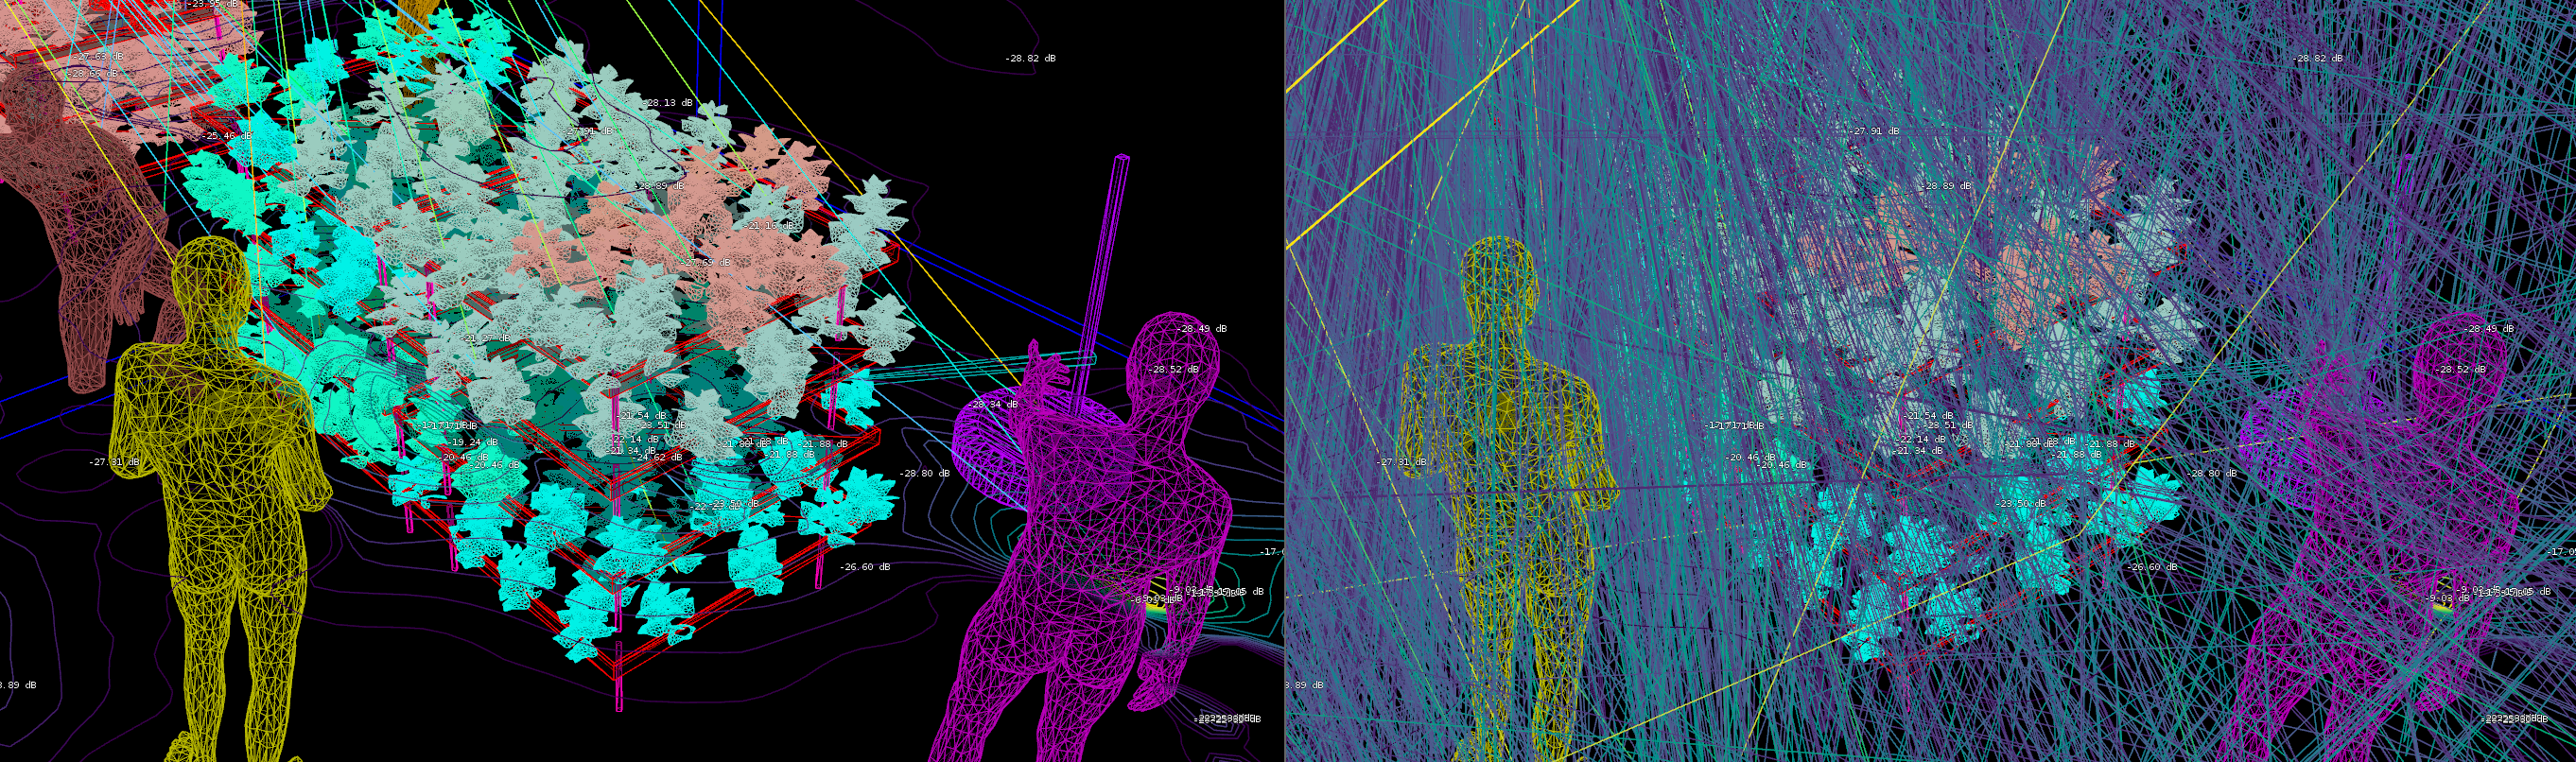
\includegraphics[width=0.98\linewidth]{figures/screenshots/snapshot combined.png}%
    % 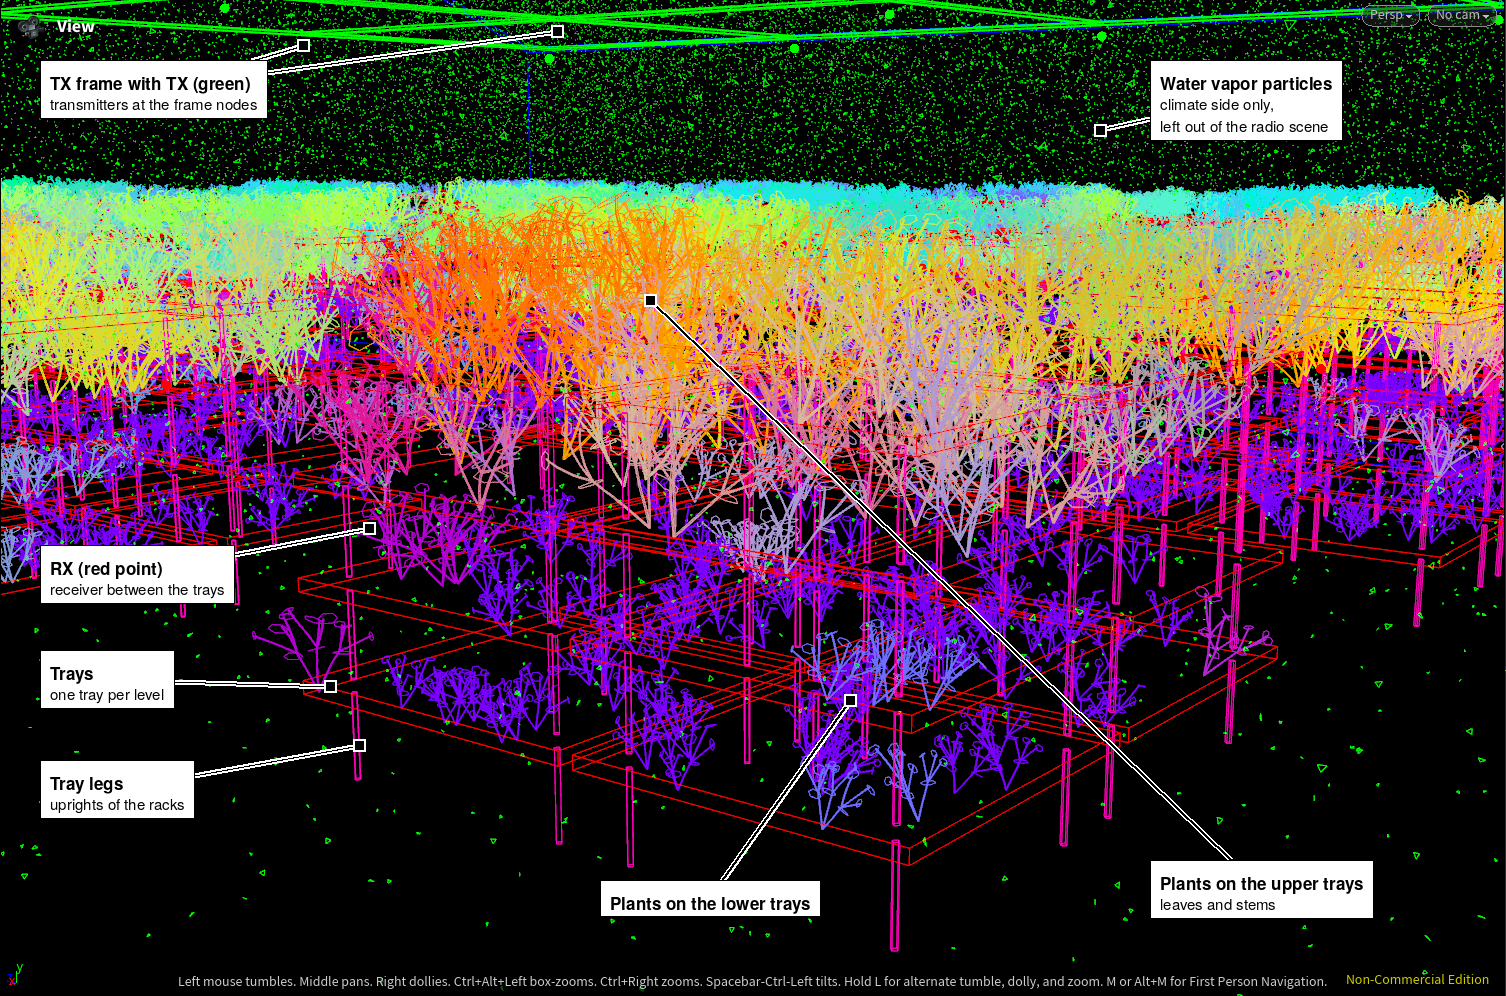
\includegraphics[width=0.5\linewidth]{figures/procedural/annotated_00bbc1c9.png}
\caption{An example cultivation scene, here with people, without and with the traced propagation paths, coloured by path delay $\tau$.}
\label{fig:usecase-paths}
\end{figure}

\emph{Sensor Node and Gateway Locations. }
Each stage is a bed of 18 plants with one sensor node per plant, attached \SI{2}{cm} from leaves, stems, and trays, so its own plant does not trigger the \SI{1}{cm} segment limit (\cref{sec:solver}). Sensor nodes with another surface within \SI{1}{cm} towards a gateway are excluded, up to three of the 18 in stage 4. Gateways \SI{2}{m} above the trays, facing down, power the sensor nodes and collect their reports: one by default, and 1 to 23 when the density is swept from one per \SI{30}{m^2} to one per \SI{1}{m^2}.

\emph{Simulation and Device Settings. }
Each scene is traced with line of sight, specular reflection, refraction, and diffraction, up to eight interactions per path, $3\times10^{6}$ samples and at most $10^{5}$ paths per transmitter, and seed 42. The sensor nodes use half-wave dipoles aligned with the main stem; the gateway uses a vertically polarised TR 38.901 element pattern. Sensor nodes are traced as transmitters; with fixed antennas, reciprocity lets the same gains serve the power transfer and the uplink. The gateways provide \SI{30}{dBm} in total at \SI{915}{MHz}; several gateways transmit coherently with maximum-ratio transmission (\cref{sec:returned}). The \gls{ble} uplink uses \SI{0}{dBm} at the sensor node, a sensitivity of \SI{-95}{dBm} at the gateway, and a \SI{10}{dB} reserve. Two commercial harvesters are compared at the same RF powers (\cref{fig:harvester_efficiency}): the e-peas AEM40940, designed for low input powers, and the Powercast P1110B, designed for higher ones. Their DC output is modelled by quadratic fits to the curves of~\cite{ambient6g}. No power is harvested below the lowest data point, at \SI{-20}{dBm} for the AEM40940 and \SI{-5}{dBm} for the P1110B, or where a fit is negative. As the curves are given at a single output voltage, the time to charge a \SI{346}{\micro\farad} buffer from \SI{0.05}{V} to the maximum storage voltage of \SI{4.5}{V} for the AEM40940, and to the maximum output voltage of \SI{4.2}{V} for the P1110B, is approximated at constant power as $t=C\,(V_1^2-V_0^2)/(2P_{\mathrm{DC}})$, neglecting leakage and cold start.

% , $P_{\mathrm{DC}}=aP_{\mathrm{RF}}^2+bP_{\mathrm{RF}}+c$ with both powers in microwatts, obtained by minimising the squared relative error: $(a,b,c)=(-2.04\cdot10^{-5},\,0.268,\,-2.19)$ for the AEM40940 and $(-1.81\cdot10^{-6},\,0.701,\,-189)$ for the P1110B. The fits are used within the datasheet range, which starts at \SI{-20}{dBm} for the AEM40940 and at \SI{-5}{dBm} for the P1110B; below it, and where a fit is negative, no power is harvested. Leakage and storage losses are not included.

% Read the original CSV directly; select each curve by its harvester column.
% text indicator handles commas inside the quoted series descriptions.
% RF input power is read directly from the level_dbm column.
\begin{figure}[t]
\centering
\pgfplotstableread[col sep=comma,text indicator="]
  {figures/harvester-chart-data.csv}\harvesterchartdata
\begin{tikzpicture}
\pgfplotsset{
  harvester series/.style={
    x filter/.code={
      \pgfplotstablegetelem{\coordindex}{harvester}\of\harvesterchartdata
      \edef\currentharvester{\pgfplotsretval}%
      \edef\selectedharvester{#1}%
      \ifnum\pdfstrcmp{\currentharvester}{\selectedharvester}=0
      \else
        \def\pgfmathresult{nan}%
      \fi
    },
    unbounded coords=discard,
    filter discard warning=false,
  },
}
\begin{axis}[
  width=\columnwidth,
  height=3.5cm,
  font=\footnotesize,
  xlabel={RF input power (dBm)},
  ylabel={Efficiency (\%)},
  label style={font=\footnotesize},
  tick label style={font=\scriptsize},
  xmin=-22, xmax=10,
  ymin=0, ymax=70,
  xtick={-25,-20,-15,-10,-5,0,5,10},
  ytick={0,20,...,60},
  grid=major,
  major grid style={draw=black!12},
  axis line style={draw=black!70},
  tick align=outside,
  tick pos=left,
  legend cell align=left,
  legend style={
    at={(0.03,0.97)}, anchor=north west,
    font=\scriptsize,
    draw=none, fill=white, fill opacity=0.9, text opacity=1,
    nodes={scale=1,transform shape},
    row sep=1pt,
  },
]
\addplot+[line width=0.9pt,draw={rgb,255:red,117;green,112;blue,179},solid,mark=*,mark size=1.3pt,harvester series=AEM40940]
table[x=level_dbm,y=efficiency] {\harvesterchartdata};
\addlegendentry{AEM40940}

\addplot+[line width=0.9pt,draw={rgb,255:red,217;green,95;blue,2},dashed,mark=square*,mark repeat=7,mark size=1.4pt,harvester series=P1110B]
table[x=level_dbm,y=efficiency] {\harvesterchartdata};
\addlegendentry{P1110B}

% \addplot+[line width=0.9pt,draw={rgb,255:red,27;green,158;blue,119},densely dotted,mark=triangle*,mark repeat=7,mark size=1.6pt,harvester series=SMS7630005LF]
% table[x=level_dbm,y=efficiency] {\harvesterchartdata};
% \addlegendentry{Low-power rectifier}

\end{axis}
\end{tikzpicture}
\caption{RF-to-DC efficiencies from the AMBIENT-6G harvester dataset~\cite{ambient6g}, at \SI{921}{MHz} for the AEM40940 and \SI{915}{MHz} for the P1110B.}
\label{fig:harvester_efficiency}
\end{figure}


\subsection{Deployment Results}

\begin{table}[t]
\caption{Results per growth stage for cherry tomato with one gateway, for the same 18 sensor nodes in every stage: median and worst path gain and median RF power at \SI{915}{MHz} (which, unlike the gain, includes fast fading), worst \gls{ble} margin at \SI{2.437}{GHz} beyond the \SI{10}{dB} reserve, and the number of sensor nodes whose harvester charges the buffer within one hour. One sensor node of stage 4 has no path to the gateway; it counts as not charged and is left out of the worst gain and margin.}
\label{tab:usecase}
\centering\footnotesize
\setlength{\tabcolsep}{3.5pt}
\begin{tabular}{@{}rrrrrrr@{}}
\toprule
 & \multicolumn{2}{c}{Gain (dB)} & \gls{ble} & $P_{\mathrm{RF}}$ & \multicolumn{2}{c}{Within \SI{1}{h} (of 18)} \\
\cmidrule(lr){2-3}\cmidrule(l){6-7}
Stage & Median & Worst & (dB) & (dBm) & AEM40940 & P1110B \\
\midrule
0 & $-36.1$ & $-48.7$  & $24.3$  & $-6.1$  & 17 & 9 \\
1 & $-47.9$ & $-57.8$  & $14.4$  & $-19.9$ & 8  & 1 \\
2 & $-51.4$ & $-59.2$  & $8.7$   & $-21.6$ & 7  & 1 \\
3 & $-52.5$ & $-66.9$  & $7.6$   & $-24.2$ & 5  & 1 \\
4 & $-64.3$ & $-102.0$ & $-20.4$ & $-36.9$ & 1  & 0 \\
\bottomrule
\end{tabular}
\end{table}

\Cref{tab:usecase} summarises the growth stages of the frequency sweep at \SI{915}{MHz}. Growth dominates: from stage 0 to stage 4, the median gain drops by \SI{28}{dB} and the median RF power from \SI{-6.1}{dBm} to \SI{-36.9}{dBm}. Over all stages, the median gain is \SI{-52.0}{dB} at \SI{915}{MHz} (\SI{-51.4}{dB} at \SI{868}{MHz}) and drops by \SI{10.1}{dB} at \SI{2.437}{GHz} and by \SI{18.3}{dB} at \SI{5.18}{GHz}, which is \SIlist{1.6;3.3}{dB} more than free-space scaling: the canopy attenuates more at higher frequencies.

Energy limits the sensor nodes first, and it depends on the harvester. With the AEM40940, whose data start at \SI{-20}{dBm}, 17 of the 18 sensor nodes charge the buffer within one hour in stage 0, but only 8 in stage 1 and a single one in stage 4. The P1110B needs \SI{-5}{dBm} and charges 9 sensor nodes in stage 0 and at most one in the later stages; above this threshold it charges the buffer within minutes, so its counts are set by the input threshold, not by the target voltage. The \gls{ble} uplink keeps at least \SI{7.6}{dB} beyond the reserve up to stage 3, but in stage 4 the worst sensor node falls \SI{20.4}{dB} short and one has no path at all.

More gateways help while the canopy is open. With 23 coherently combined gateways, all 18 sensor nodes charge within one hour with the AEM40940 in stages 0 to 2, against 17, 9, and 7 with one gateway in the same sweep, but in stage 4 only 2 of the 16 sensor nodes that are not excluded do: the dense canopy, not the number of gateways, then limits power delivery. The species matters as much as the stage: the median RF power under butterhead lettuce stays near \SI{-17}{dBm} in every stage, whereas it falls by \SI{11}{dB} for sweet basil, \SI{18}{dB} for strawberry, and \SI{29}{dB} for cherry tomato. Leaf water content between \SIlist{20;90}{\percent} changes the median gain by at most \SI{2}{dB}, as \SI{0.3}{mm} leaves are electrically thin, and the number of charged sensor nodes by at most two. Runs with identical inputs and seed are not bit-identical on the GPU; between such runs, the count differs by at most one sensor node.


\balance
\section{Discussion and Conclusions}
\label{sec:conclusion}
\housionna{} connects procedural scene generation, GPU radio ray tracing, batch execution, inspection of paths and radio maps in Houdini and a web viewer, and an application engine for communication and \gls{wpt} metrics. This provides a practical basis for studying the RF infrastructure serving agricultural sensors across changing crop configurations. In the use case, canopy growth, species, and gateway density changed which sensor nodes could be powered, whereas leaf water content barely did. One solver limitation holds independently of the scene: the path solver discards paths through closed structures thinner than \SI{1}{cm}, which affects sensor nodes mounted directly on leaves.

\emph{Towards an Agricultural Digital Twin. }\label{sec:twin}
Procedural simulation supports controlled comparisons and reproducible scenario generation, but a digital twin also requires a maintained relationship with the physical environment. In this setting, that relationship would connect observed crop geometry and operating conditions to calibrated RF materials, antenna models, and validated predictions. Periodic updates could then test whether an existing network remains adequate as the crop develops.

None of the results has yet been compared with measurements. Three limits are particularly relevant. First, the present vegetation materials are provisional, and surface-based canopy representations need evaluation across the intended frequencies, in particular for thin leaves; stems are not modelled. Second, the antenna models are ideal patterns: they do not capture plant-mounted antenna detuning or efficiency, and each device has a single antenna element, so array-based power delivery is not modelled. Third, a sequence of static scenes does not provide continuous state estimation or validated dynamic sensing.

Sionna RT supports differentiable modelling~\cite{hoydis2023,aoudia2025}, but the file-based wrapper described here does not provide an end-to-end differentiable Houdini pipeline. Gateway placement can be compared by searching subsets of candidate positions on precomputed channels; gradient-based material fitting or continuous placement would need a deliberate integration with the solver. Protocol performance, backscatter modulation, and RF crop inference likewise remain separate modelling tasks.

% The broader \hyropa{} programme also covers optical propagation; optical energy harvesting and hybrid links are possible extensions.

% \subsection{Remote Canopy Sensing}
% The remote-sensing application considered here is proximal RF observation of crop canopies. For a channel feature vector $\mathbf{z}$, one can investigate the response
% \begin{equation}
%  \Delta\mathbf{z}
%  =\mathbf{z}(\boldsymbol{\theta}+\Delta\boldsymbol{\theta})
%   -\mathbf{z}(\boldsymbol{\theta}),
% \end{equation}
% where $\boldsymbol{\theta}$ describes crop geometry and calibrated material parameters. Candidate features include link attenuation, delay spread, and frequency-selective response. In \housionna{}, $\boldsymbol{\theta}$ corresponds to the parameters of a batch sweep, so $\Delta\mathbf{z}$ follows from neighbouring work items of the same batch.


% Sensitivity is only the first step. Similar channel changes can arise from plant growth, water content, antenna displacement, people, or equipment; since people and robots can be placed in the scenes, their effect can be simulated alongside that of the crop. An inference study must quantify these ambiguities against independent canopy observations.

% \emph{Future Work. }
% The next scientific step is to validate canopy representations and material parameters, then evaluate communication, energy, and sensing metrics against physical observations.


% \section*{Acknowledgment}

\printbibliography%

\end{document}
